\documentclass[12pt,a4paper,oneside]{report}
\usepackage[T1]{fontenc}
\usepackage{mathptmx}
\usepackage[left=30mm,right=25mm,top=25mm,bottom=25mm]{geometry}

\usepackage{titlesec}
\usepackage{fancyhdr}
\setlength{\headheight}{30pt}
\setlength{\headsep}{12pt}


\usepackage{graphicx,array,longtable,pdflscape,setspace}
\usepackage[hidelinks]{hyperref}
\onehalfspacing
\setlength{\parindent}{0pt}
\setlength{\parskip}{4pt}
\setcounter{tocdepth}{1}
\renewcommand{\contentsname}{Table of Contents}
\newcommand{\institutionlogo}[1]{\IfFileExists{amrita-logo.png}{
\includegraphics[width=#1]{amrita-logo.png}}{\fbox{\parbox{#1}{\centering Amrita Vishwa Vidyapeetham\\Place amrita-logo.png beside this file}}}}
\newcommand{\ProjectTitle}{Secure and Role-Aware Explainable Occupant Tracking in Multi-Building Indoor Smart Spaces}
\fancypagestyle{project}{%
  \fancyhf{}
  \fancyhead[C]{\parbox{\textwidth}{\centering\small\nouppercase{\ProjectTitle}}}
  \fancyfoot[C]{\thepage}
  \renewcommand{\headrulewidth}{0.4pt}
}
% Preliminary pages show only a page number.
\fancypagestyle{plain}{%
  \fancyhf{}
  \fancyfoot[C]{\thepage}
  \renewcommand{\headrulewidth}{0pt}
}
\newcommand{\EnableProjectHeaders}{%
  \pagestyle{project}%
  % report uses plain style on chapter-opening pages.
  \fancypagestyle{plain}{%
    \fancyhf{}
    \fancyhead[C]{\parbox{\textwidth}{\centering\small\nouppercase{\ProjectTitle}}}
    \fancyfoot[C]{\thepage}
    \renewcommand{\headrulewidth}{0.4pt}
  }%
}
\titlespacing*{\chapter}{0pt}{0pt}{16pt}
\titlespacing*{\section}{0pt}{10pt}{4pt}
\titlespacing*{\subsection}{0pt}{8pt}{3pt}
\titlespacing*{\subsubsection}{0pt}{6pt}{3pt}
\raggedbottom
\begin{document}
\pagestyle{empty}

{\centering \Large\bfseries \ProjectTitle{}\par}
{\centering Project report submitted in partial fulfilment of the requirements for the award of the degree of\par}
{\centering \textbf{BACHELOR OF TECHNOLOGY}\par}
{\centering in\par}
{\centering \textbf{COMPUTER SCIENCE AND ENGINEERING}\par}
{\centering Submitted by\par}
{\centering \fontsize{14}{18}\selectfont
Ajith Ashok \quad AM.U4.U4CSE23204\par}

{\centering \fontsize{14}{18}\selectfont
Arjun Rajesh \quad AM.U4.U4CSE23208\par}

{\centering \fontsize{14}{18}\selectfont
D Aditya Kiran \quad AM.U4.U4CSE23215\par}

{\centering \fontsize{14}{18}\selectfont
Yadhu Vipin Madhilakath Madathil \quad AM.U4.U4CSE23270\par}

{\centering \fontsize{14}{18}\selectfont
Under the guidance of\par
Dr. Lakshmi Mohan\par
Assistant Professor\par}

{\centering \institutionlogo{4.5in}\par}

{\centering \textbf{AMRITA SCHOOL OF COMPUTING}\par}
{\centering \textbf{AMRITA VISHWA VIDYAPEETHAM}\par}
{\centering \textbf{AMRITAPURI CAMPUS}\par}
{\centering \textbf{KOLLAM 690525}\par}
{\centering \textbf{NOVEMBER 2026}\par}


\clearpage
{\centering \institutionlogo{3.7in}\par}
{\centering \textbf{DEPARTMENT OF COMPUTER SCIENCE AND ENGINEERING}\par}
{\centering Amrita School of Computing, Amritapuri Campus\par}
{\centering \Large\bfseries BONAFIDE CERTIFICATE\par}
This is to certify that the project report entitled ``\ProjectTitle{}'', submitted by Ajith Ashok (AM.U4.U4CSE23204), Arjun Rajesh (AM.U4.U4CSE23208), D Aditya Kiran (AM.U4.U4CSE23215) and Yadhu Vipin Madhilakath Madathil (AM.U4.U4CSE23270), in partial fulfilment of the requirements for the award of the degree of Bachelor of Technology in Computer Science and Engineering at Amrita Vishwa Vidyapeetham, is a bonafide record of the work carried out by them under my guidance and supervision at Amrita School of Computing, Amritapuri, during Semester 7 of the academic year 2026 - 2027.

\begin{tabular}{p{.46\textwidth}p{.46\textwidth}} Dr. Lakshmi Mohan & \phantom{X} \\ Project Guide & Project Coordinator \\ Signature \hrulefill & Signature \hrulefill \\[20pt] \phantom{X} &  \\ Chairperson, CSE & Reviewers \\ Signature \hrulefill & Signature \hrulefill \end{tabular}
\\
\\ 
\\ Place: Amritapuri\\
Date: 4 November 2026 
\clearpage
\thispagestyle{empty}

{\centering
\institutionlogo{3.7in}\par
\vspace{0.4cm}
\textbf{DEPARTMENT OF COMPUTER SCIENCE AND ENGINEERING}\par
Amrita School of Computing, Amritapuri Campus\par
\vspace{0.6cm}
{\Large\bfseries DECLARATION\par}
}

\vspace{0.5cm}

\noindent
We, Ajith Ashok (AM.U4.U4CSE23204),
Arjun Rajesh (AM.U4.U4CSE23208),
D Aditya Kiran (AM.U4.U4CSE23215) and
Yadhu Vipin Madhilakath Madathil (AM.U4.U4CSE23270),
hereby declare that the project entitled
``\ProjectTitle{}'' is a record of our original work
carried out under the guidance of Dr. Lakshmi Mohan, Assistant Professor,
Department of Computer Science and Engineering,
Amrita Vishwa Vidyapeetham, Amritapuri.
To the best of our knowledge, this work has not formed the
basis for the award of any degree, diploma, fellowship or
similar qualification to any candidate at any university.
All sources and contributions of others have been
appropriately acknowledged.

\vspace{0.5cm}

\noindent
Place: Amritapuri\\
Date: 4 November 2026

\vspace{0.7cm}

\noindent
\begin{tabular}{@{}p{0.60\textwidth}p{0.34\textwidth}@{}}
\textbf{Student details} & \textbf{Signature of the student} \\[14pt]

Ajith Ashok\newline
AM.U4.U4CSE23204
& \rule{0.30\textwidth}{0.4pt} \\[18pt]

Arjun Rajesh\newline
AM.U4.U4CSE23208
& \rule{0.30\textwidth}{0.4pt} \\[18pt]

D Aditya Kiran\newline
AM.U4.U4CSE23215
& \rule{0.30\textwidth}{0.4pt} \\[18pt]

Yadhu Vipin Madhilakath Madathil\newline
AM.U4.U4CSE23270
& \rule{0.30\textwidth}{0.4pt}
\end{tabular}

\vspace{0.8cm}

\noindent
\textbf{Project Guide:} Dr. Lakshmi Mohan

\vspace{0.5cm}

\noindent
\textbf{Signature of the Project Guide:}
\rule{4cm}{0.4pt}

\clearpage

\clearpage
% Arabic numbering continues through the preliminary pages and chapters.
\clearpage
\pagenumbering{roman}
\pagestyle{plain}

\phantomsection
\addcontentsline{toc}{chapter}{Acknowledgement}
{\centering \Large\bfseries ACKNOWLEDGEMENT\par}
We thank our guide, Dr. Lakshmi Mohan, for proposing the problem, for the Distributed State Transition System framework on which this work builds, and for guiding every review from the first literature survey to the final evaluation. Her comments at the mid-review shaped the role-based access control, the explainability and the security work reported here.

We are grateful to the Department of Computer Science and Engineering and the Amrita School of Computing, Amritapuri Campus, for the computing facilities and the review process that kept the project on schedule. We also thank the authors of the open datasets and models we used, CASIA-WebFace, the Real-World Masked Face Dataset (RMFRD) and the InsightFace models, whose public release made this evaluation possible.

Finally, we thank our team members for the shared effort across the parts of the project: the routing and pipeline, the query, access-control and security layers, the explanation layer and the dashboard.

\clearpage
\phantomsection
\addcontentsline{toc}{chapter}{Abstract}
{\centering \Large\bfseries ABSTRACT\par}
Multi-building campuses need to recognise and follow people across buildings, but keeping every face template in one central store concentrates sensitive biometric data, while keeping the templates apart makes it hard to find the building that knows a visitor. This project extends the Distributed State Transition System (DSTS) framework to decentralised multi-building occupant identification and tracking, with secure, role-based and explainable access to the results. Each building keeps its own gallery and publishes only a Bloom filter built from locality-sensitive-hash (LSH) codes of its occupants' face embeddings. A capture that is not recognised locally is routed to a short list of likely buildings, which verify it by angular-distance voting. A dynamic visitor database, per-state probabilistic tracking, two-layer role-based access control with a class-teacher model, sealed inter-building transfers and explanations redacted to the caller's disclosure level complete the system. It is evaluated on 550 simulated occupants in 11 buildings (500 from CASIA-WebFace and 50 masked people from the real-world RMFRD dataset) over 11,000 events per simulated day, against a centralised search, and averaged over five random populations. The decentralised pipeline identifies 91.5\% of events against 92.2\% for the central search while touching 10.3\% of the galleries; building-level state F1 is 0.950. Unmasked people are identified 94.8\% of the time and masked people 59.1\%. The uncertainty flags attached to answers catch 74\% of wrong identifications at a cost of about 8\% extra latency, and 575 automated tests cover the policy, secure-transfer and explanation layers. The network, cameras and certificate authority are simulated, so the work demonstrates the design and its accuracy rather than a hardened deployment.

Keywords: Occupant identification and tracking; Distributed state transition system; Locality-sensitive hashing; Bloom filter; Role-based access control; Explainable queries; Masked face recognition


\clearpage
\tableofcontents
\clearpage
\phantomsection
\addcontentsline{toc}{chapter}{List of Figures}
\listoffigures
\clearpage
\phantomsection
\addcontentsline{toc}{chapter}{List of Tables}
\listoftables
\clearpage
\pagenumbering{arabic}
\pagestyle{plain}
\EnableProjectHeaders
\chapter{Introduction}
\section{Background and motivation}
Smart spaces use cameras, sensors and computing to observe who is where and to support occupant-specific services such as access, scheduling and safety \cite{ref6,ref7,ref26}. On a university campus or a corporate estate these services span many buildings, so the system must keep identifying and following a person as they walk from one building to the next. Camera networks for indoor tracking are well studied \cite{ref1,ref2,ref3,ref4,ref5}, but the identity question changes when the space has several buildings: a person registered in one building is a \emph{visitor} in every other, and the building that captures the face does not hold that person's reference photos.

There are two obvious designs. A \emph{centralised} design keeps every person's reference embeddings in one store and searches all of them for every capture. It is simple and accurate, but it concentrates biometric data, which cannot be reissued if it leaks, and it makes one server the single point of failure and of attack. A \emph{distributed} design keeps each building's reference data in that building. This respects the locality of the data, but a visitor's home building is unknown, so the capturing building must either contact every other building for every unrecognised face or share reference embeddings between buildings \cite{ref6}. The base paper that this project extends, the Distributed State Transition System (DSTS) of Mohan and Menon \cite{ref6}, resolves visitors through a central master list.

A second gap concerns the people who ask questions of the tracking data. The same data that lets a Dean find a lost visitor also lets any user follow any other person, so the system must decide who may see whom, and at what precision \cite{ref21}, and must be able to show why an answer was given. Access control for tracking queries and explanations of the answers are rarely treated together with distributed identification.

This project therefore combines three things in one system: (i) decentralised identification and tracking in which only a one-way Bloom filter leaves a building until a match is confirmed; (ii) role-based, privacy-aware querying with a two-layer policy; and (iii) explanations that justify both the access decision and the tracking evidence behind each answer. A first, narrower study of the routing step alone has been written up as a conference-style manuscript \cite{ref28}; this report covers the complete system, including state tracking, access control, security, explanations and a masked-face building.

\textbf{Relevant Sustainable Development Goals.} The work maps to three goals of the 2030 Agenda \cite{ref27}: \emph{SDG~9} (target 9.1, resilient infrastructure), because there is no central biometric store to lose; \emph{SDG~11} (target 11.7, safe and inclusive spaces), because occupants can be located for safety while their data is protected from misuse such as stalking; and \emph{SDG~16} (target 16.6, accountable and transparent institutions), because every access decision is audited and every answer is explained.

\section{Objectives}
The objectives, each linked to how it is evaluated and to its deliverable, are given in Table~\ref{tab:objectives}.

\begin{table}[htbp]
\centering
\caption{Objectives, evaluation methods and deliverables}\label{tab:objectives}
{\small\setlength{\tabcolsep}{4pt}\renewcommand{\arraystretch}{1.2}
\begin{tabular}{|p{0.6cm}|p{4.4cm}|p{5.2cm}|p{3.6cm}|}\hline
\textbf{\#} & \textbf{Objective} & \textbf{Evaluation method} & \textbf{Deliverable}\\\hline
1 & Extend the DSTS framework to distributed multi-building identification and tracking & Event identification precision and recall; state-level precision and recall over every state (Sections~\ref{sec:res-events}, \ref{sec:res-state}) & Pipeline, building nodes, BSTS state store\\\hline
2 & Provide an RBAC query interface for Dean, Teacher and Student roles & Every policy cell tested; access matrix checked against the expected decisions (Section~\ref{sec:res-security}) & Two-layer policy, FastAPI server, dashboard\\\hline
3 & Return explainable responses that justify the access decision and the tracking evidence & Faithfulness and no-leakage tests; flag precision and recall against ground truth; latency overhead (Section~\ref{sec:res-expl}) & Explanation model, redaction, ``Why this answer'' card\\\hline
4 & Design LSH + Bloom-filter routing for decentralised visitor lookup & Routing recall; gallery touched per lookup; accuracy against a centralised search; effective false-positive rate (Sections~\ref{sec:res-events}, \ref{sec:res-visitors}, \ref{sec:res-bloom}) & Enrolment, routing and verification modules\\\hline
5 & Secure the system: sealed transfers, role-based filtering, audit logging & Tamper, replay, wrong-sender and fail-closed tests; login lockout tests (Section~\ref{sec:res-security}) & secure\_\allowbreak transfer and access\_\allowbreak control packages\\\hline
6 & Evaluate tracking precision and recall, communication cost and explanation quality & TP/FP/FN/TN per cohort and level; five seeds; centralised baseline; explanation measurements (Chapter~\ref{ch:results}) & Evaluation scripts and result tables\\\hline
\end{tabular}}
\end{table}

\section{Scope and constraints}
\textbf{Intended users.} Campus administrators (Deans), faculty (Teachers) and students; each sees tracking data only as their role and relationship allow. \textbf{Included functions.} Face-embedding based identification of registered occupants and of visitors across buildings; probabilistic zone-level tracking; thirteen query templates (Q1--Q13) and a full-trajectory query; role-based disclosure; explanations; secure inter-building exchange; a web dashboard; and a centralised baseline for comparison.

\textbf{Exclusions and assumptions.} The system works on face embeddings produced by a pretrained model; it does not train a face model or process live video. Cameras, the network between buildings and the certificate authority are simulated in one process, and the test photos are replayed as camera events. Zones are a fixed nine-zone layout per building. Every visitor is registered in some other building; people registered nowhere (unknown visitors) are future work. \textbf{Constraints.} All experiments run on a laptop CPU and are reproducible from a population seed.

\section{Project report organization}
Chapter~2 states the problem, Chapter~3 reviews fourteen related works, and Chapter~4 lists the requirements. Chapter~5 presents the design and its parameters, Chapter~6 the evaluation, results, comparison and limitations, and Chapter~7 the conclusion and future work. The references and an appendix on reproducibility follow.

\clearpage
\chapter{Problem Definition}
\section{Problem statement}
\textbf{Problem.} Identify and track occupants across a wide-area, multi-building indoor environment while giving secure, role-based and explainable access to where they are and have been, and justify both the access decisions and the tracking evidence behind each answer.

\textbf{Stakeholders and consequences.} Occupants, Deans, Teachers, Students and auditors are affected. Centralised identification means one breach exposes everyone's biometric data; distribution without routing costs a request to every building per unrecognised face; uncontrolled access turns tracking into a stalking tool; and unexplained answers cannot be audited.





\section{Existing system and limitations}
Existing indoor tracking systems use cameras, radio signals or both \cite{ref1,ref2,ref9}. Edge-camera frameworks localise and track people accurately inside one site \cite{ref1,ref2,ref5}, and distributed trackers associate targets across cameras with consensus filtering or shared target tables \cite{ref3,ref4}. These systems stay within one site. They do not say how a person registered elsewhere is identified or who may query the locations.

The DSTS framework \cite{ref6} models a multi-building environment as states, events and transition functions and resolves visitors through a centralised master list. Bloom filters have protected biometric templates \cite{ref10,ref11} and found web proxies \cite{ref13}, but none of the reviewed work combines approximate, similarity-based routing of a face to a building with role-based access control and explanations.



\textbf{Gap.} Four gaps remain: (i) identity discovery across separate buildings without sharing galleries; (ii) evidence that LSH with Bloom filters can route biometric visitors accurately; (iii) role-based control over tracking queries; and (iv) explanations for access decisions and tracking answers. This project addresses all four.

\clearpage
\chapter{Literature Review}
\section{Review scope and selection}
Fourteen works (references 1--6, 8 and 10--16) were reviewed in twelve groups (Section~\ref{sec:lit-desc}); they are cited by their reference number throughout the report. The search covered indoor occupant tracking with camera and RF sensing, multi-camera association, state-transition models of smart spaces, privacy-preserving biometrics and Bloom-filter indexing, and similarity search with locality-sensitive hashing. Search keywords were: ``indoor localization camera network edge'', ``distributed multi-camera multi-target tracking'', ``smart space state transition'', ``Bloom filter biometric'', ``locality sensitive hashing'' and ``masked face recognition dataset''.

The publication period is 1970 to 2026: recent works (2020--2026) on tracking and privacy-preserving biometrics were chosen for the problem context, and foundational works on Bloom filters and hashing were included because the routing mechanism is built on them. A work was selected if it is a primary source (a journal article, conference paper or preprint), is directly relevant to tracking, identity discovery, hashing-based routing, or the models used in this project, and gives enough detail to describe its approach and evaluation. Works [1]--[5] are the mid-review set; [6] is the base paper that this project extends. The remaining references (the datasets, face models, access-control model and cryptographic standards used in Chapters 4 and 5) are cited where they are used and are not reviewed here.

\section{Descriptive review of literature works}\label{sec:lit-desc}
Each group below gives one connected paragraph covering the problem or objective, the proposed contribution and approach, the study context, the evaluation criteria, the key findings and the limitations that leave a gap for this project. Table~\ref{tab:literature} compares all of them.

\clearpage
\subsection{Group identification and localization with privacy-preserving edge cameras}
Hegde et al. (2024) in ``Indoor group identification and localization using privacy-preserving edge computing distributed camera network'' \cite{ref1} investigate how to find when and where groups form in an indoor therapeutic space of about 1,700~m$^2$. The work proposes a pipeline that takes noisy positions and orientations of people, estimated from sparsely placed multi-view edge cameras running a lightweight two-dimensional pose detector, and groups them. The study is situated in a therapeutic built environment with seven participants over 35-minute sessions in groups of two to seven. The authors assess it with precision, recall and F1 for group identification and mean absolute error for group localization. They report F1 of up to about 90\% and a localization error of 1.25~m, with raw images kept off the network because the edge devices extract the features. The limitations are that the unit of identification is a group and not an individual, and that the study covers one space; it says nothing about identifying a person who is registered elsewhere.

\subsection{Indoor localization and multi-person tracking with sparse edge cameras}
Kwon et al. (2023) in ``A feasibility study on indoor localization and multiperson tracking using sparsely distributed camera network with edge computing'' \cite{ref2} ask whether people can be localized and tracked over a large indoor site with few, low-cost cameras. They deploy 39 edge camera units, each running pose estimation on a Google Coral accelerator, in a therapeutic space of roughly 1,700~m$^2$, and track people from the pose output. The evaluation reports localization error, multiple-object tracking accuracy, tracking precision, identity switches and body-orientation error, with an average localization error of about 1.4~m and a tracking accuracy of about 88.6\%. The framework tracks anonymous people inside one site and does not attempt cross-building identity discovery, access control or explanations.

\clearpage
\subsection{Distributed multi-camera multi-target association}
Yang et al. (2022) in ``Distributed multi-camera multi-target association for real-time tracking'' \cite{ref3} address real-time association of targets across cameras without a central server. They propose a target-management module in which cameras share a data structure of target labels and appearance information so that detections in different views can be matched, without camera calibration. The evaluation uses several multi-camera benchmarks and an own mobile-camera dataset and reports multi-camera tracking accuracy, IDF1, false positives, false negatives and identity switches. The work improves association, but it keeps no probabilistic state of who is in which building and does not identify where a visitor comes from.

\subsection{Distributed multi-target tracking in camera networks}
Casao et al. (2021) in ``Distributed multi-target tracking in camera networks'' \cite{ref4} study tracking of several people with a network of cameras that exchange information only with neighbours. Their approach combines a distributed-consensus Kalman filter with a re-identification network and a distributed tracker manager that handles cross-camera association. They compare against centralised trackers on public multi-camera datasets using tracking accuracy, IDF1-type scores and bandwidth, and report better accuracy and lower bandwidth than the centralised methods they compare with. The gap is that the system tracks within one camera network and has no model of buildings, registered occupants and visitors.

\clearpage
\subsection{Real-time multi-person multi-camera tracking at the edge}
Gaikwad and Karmakar (2021) in ``Smart surveillance system for real-time multi-person multi-camera tracking at the edge'' \cite{ref5} build an end-to-end pipeline of detection, tracking and re-identification that runs on an NVIDIA Jetson TX2 edge device. It is evaluated on the authors' own multi-camera campus recordings, collected over a full day, and reports an IDF1 score of 90.97, about 30 frames per second and a re-identification latency of roughly 90~ms. The pipeline shows that edge tracking and re-identification are practical, but it has no formal multi-building state or query model and no decentralised handling of visitors.

\subsection{Modelling large-scale camera networks: the DSTS framework}
Mohan and Menon (2020) in ``Modelling large scale camera networks for identification and tracking: an abstract framework'' \cite{ref6} model identification and tracking in a wide-area camera network as a distributed state transition system. A state records the probability that each occupant is in each zone, an event is a recognition at a zone, and a transition function updates the state when an event occurs; each building has a building-level state transition system (BSTS). Registered occupants are recognised against their own building's database, and visitors are resolved through a centralised master list. The framework is abstract and the visitor step is the part this project replaces: the central list concentrates biometric data and every visitor lookup depends on it. The model of states, events and transitions builds on earlier work on the three Rs of cyber-physical spaces \cite{ref7}.

\clearpage
\subsection{Face recognition and tracking for security surveillance}
Nair et al. (2021) in ``Face recognition and tracking for security surveillance'' \cite{ref8} investigate identifying and following faces across surveillance cameras, including cameras with non-overlapping views. The work combines face detection and recognition with tracking so that a person recognised in one camera can be followed into the next. It shows that face recognition is a practical identity cue for tracking, which is the assumption this project relies on. As a surveillance system it is not designed around separate per-building galleries, cross-building identity discovery or role-based querying.

\subsection{Bloom filters for iris biometrics}
Rathgeb et al. (2014) in ``On application of Bloom filters to iris biometrics'' \cite{ref10} investigate how Bloom filters can hold iris templates. Representing the template as a Bloom filter makes comparison alignment-free and one-way, so that the stored template protects the biometric while still allowing identification, and the structure supports faster searches than a linear scan of templates. The work establishes that Bloom filters are a usable representation for biometric data. It targets iris codes, not face embeddings, and it protects a single database rather than routing a query among many databases.

\clearpage
\subsection{Privacy-preserving face-based crowd monitoring}
Marzani et al. (2026) in ``Head count: privacy-preserving face-based crowd monitoring'' \cite{ref11} address counting individuals across locations without revealing their faces. They combine face features, fuzzy extractors and homomorphically encrypted Bloom filters so that the same person seen in different places is counted once while the underlying biometric stays hidden. This is the closest related work to using Bloom filters for cross-location face matching. Its purpose is counting, not identification and tracking of named occupants, and it has no role-based query layer; this project uses LSH codes and per-building Bloom filters to route a capture towards the building that holds the reference.

\subsection{Space/time trade-offs in hash coding}
Bloom (1970) in ``Space/time trade-offs in hash coding with allowable errors'' \cite{ref12} introduces the Bloom filter: a bit array and several hash functions that answer ``probably in the set'' or ``definitely not in the set'', with a controllable false-positive rate and no false negatives. The analysis trades a small error probability for a large saving in space. This is the property the project depends on: each building can publish a compact, one-way summary of its occupants. The filter answers exact membership only, which is why locality-sensitive hashing is needed to make nearby embeddings collide; and, as Section~\ref{sec:res-bloom} shows, the analysis assumes independent items, which LSH codes are not.

\clearpage
\subsection{Summary Cache: Bloom filters for wide-area cache sharing}
Fan et al. (2000) in ``Summary Cache: a scalable wide-area web cache sharing protocol'' \cite{ref13} study how web proxies can share cache contents without flooding each other with queries. Each proxy keeps a Bloom-filter summary of the objects held by its peers and contacts only the peers whose summaries match, which sharply reduces inter-proxy messages at a small cost in false hits. The evaluation is on trace-driven simulations of proxy traffic. The same idea of summaries that tell where an item probably lives is applied here to faces, but a face capture never matches exactly, so the summaries must be built from similarity-preserving codes.

\subsection{Similarity-preserving hashing: SimHash and multi-probe LSH}
Charikar (2002) in ``Similarity estimation techniques from rounding algorithms'' \cite{ref14} shows that random-hyperplane hashing maps vectors to bits so that the probability of two vectors agreeing on a bit grows with the angle between them, which makes binary codes preserve angular similarity. Lv et al. (2007) in ``Multi-probe LSH: efficient indexing for high-dimensional similarity search'' \cite{ref15} improve recall without more hash tables by also probing the buckets that differ from the query in the least confident bits. Kirsch and Mitzenmacher (2006) show that Bloom-filter positions can be derived by double hashing with no loss in asymptotic false-positive rate \cite{ref16}. These three works supply the encoding, multi-probe lookup and hashing used in this project. They are generic indexing techniques and say nothing about biometric privacy or access control.

\clearpage
\begin{landscape}
\section{Comparison of reviewed literature}
Table~\ref{tab:literature} compares the reviewed works on the attributes used above. The gap that follows from the comparison is stated here, and the table gives the evidence. \textbf{Gap.} None of the surveyed works routes a face from a building that does not know it to the building that does, using compact similarity-preserving summaries, and none combines this with role-based access to the tracking data and with explanations of the answers. That combination is the contribution of this project.

\begingroup\small\setlength{\tabcolsep}{4pt}\renewcommand{\arraystretch}{1.25}
\begin{longtable}{|p{2.2cm}|p{2.6cm}|p{3.5cm}|p{2.7cm}|p{3.0cm}|p{2.9cm}|p{3.3cm}|}
\caption{Comparison of reviewed literature}\label{tab:literature}\\\hline
\textbf{Work and citation} & \textbf{Problem or objective} & \textbf{Approach and contribution} & \textbf{Study context} & \textbf{Evaluation criteria} & \textbf{Key findings} & \textbf{Limitations and gap}\\\hline\endfirsthead
\hline\textbf{Work and citation} & \textbf{Problem or objective} & \textbf{Approach and contribution} & \textbf{Study context} & \textbf{Evaluation criteria} & \textbf{Key findings} & \textbf{Limitations and gap}\\\hline\endhead
Work 01 \cite{ref1} Hegde et al., 2024 & Find when and where groups form indoors & Pose estimation and clustering on edge cameras & One therapeutic space, 7 people, 35 min & Precision, recall, F1, MAE & F1 up to about 90\%, MAE 1.25~m & Groups, not individuals; one site\\\hline
Work 02 \cite{ref2} Kwon et al., 2023 & Localize and track people with few cameras & 39 edge units with pose estimation & About 1,700~m$^2$ therapeutic space & Localization error, MOTA, MOTP, ID switches & About 1.4~m error, MOTA about 88.6\% & Anonymous tracking in one site\\\hline
Work 03 \cite{ref3} Yang et al., 2022 & Distributed multi-target association & Shared label and appearance table, no calibration & Benchmarks and an own mobile-camera set & MOTA, IDF1, FP/FN, ID switches & Real-time association without a server & No building-level state or visitor origin\\\hline
Work 04 \cite{ref4} Casao et al., 2021 & Distributed multi-target tracking & Consensus Kalman filter, re-ID and tracker manager & Public multi-camera datasets & MOTA/IDF1-type, bandwidth & Better than centralised in accuracy and bandwidth & One camera network; no occupants or visitors\\\hline
Work 05 \cite{ref5} Gaikwad and Karmakar, 2021 & Edge multi-person multi-camera tracking & Detection, tracking and re-ID on Jetson TX2 & Own campus recordings, one day & IDF1, FPS, re-ID latency & IDF1 90.97, about 30 FPS, about 90~ms & No multi-building state or query model\\\hline
Work 06 \cite{ref6} Mohan and Menon, 2020 & Model camera-network identification and tracking & Abstract DSTS: states, events, transitions & Abstract framework & Analytical & Formal model with building-level BSTS & Visitors via a central master list\\\hline
Work 07 \cite{ref8} Nair et al., 2021 & Face recognition and tracking & Recognition and tracking across cameras & Surveillance cameras & Recognition and tracking quality & Face is a workable identity cue & Not built around per-building galleries or access control\\\hline
Work 08 \cite{ref10} Rathgeb et al., 2014 & Protect iris templates & Bloom-filter templates & Iris databases & Comparison and speed & Alignment-free, one-way templates & Iris, not face; one database, no routing\\\hline
Work 09 \cite{ref11} Marzani et al., 2026 & Privacy-preserving crowd counting & Face features, fuzzy extractor, encrypted Bloom filters & Multi-location counting & Counting accuracy, privacy & Counts people without revealing faces & Counts, does not identify; no roles\\\hline
Work 10 \cite{ref12,ref16} Bloom, 1970; Kirsch and Mitzenmacher, 2006 & Compact set membership & Bit array and hash functions; double hashing & Theory & False-positive rate, space & No false negatives; tunable error & Exact membership only; assumes independent items\\\hline
Work 11 \cite{ref13} Fan et al., 2000 & Share web caches cheaply & Bloom-filter summaries of peers & Proxy traces & Messages, hit ratio & Far fewer inter-proxy messages & Exact keys, not similar faces\\\hline
Work 12 \cite{ref14,ref15} Charikar, 2002; Lv et al., 2007 & Similarity-preserving hashing & Random hyperplanes; multi-probe lookup & Theory, similarity search & Recall, tables needed & Angle-preserving codes; fewer tables & Generic; no privacy or access control\\\hline
\end{longtable}\endgroup
\end{landscape}
\clearpage

\clearpage
\chapter{Requirements}
\section{Functional requirements}
Table~\ref{tab:fr} lists the functional requirements with their actors, inputs and outputs, and the acceptance criterion used to check each one.

{\small\setlength{\tabcolsep}{4pt}\renewcommand{\arraystretch}{1.2}
\begin{longtable}{|p{1.0cm}|p{4.0cm}|p{2.0cm}|p{3.4cm}|p{4.2cm}|}
\caption{Functional requirements}\label{tab:fr}\\\hline
\textbf{ID} & \textbf{Requirement} & \textbf{Actor} & \textbf{Input $\rightarrow$ output} & \textbf{Acceptance criterion}\\\hline\endfirsthead
\hline\textbf{ID} & \textbf{Requirement} & \textbf{Actor} & \textbf{Input $\rightarrow$ output} & \textbf{Acceptance criterion}\\\hline\endhead
FR1 & Recognise a registered occupant against the building's own gallery & Camera event & Embedding $\rightarrow$ identity or abstain & Accepted when at least 12 of 20 references agree within 80.43$^{\circ}$\\\hline
FR2 & Route an unrecognised capture to likely buildings with Bloom filters, then verify there & Building node & Embedding $\rightarrow$ shortlist, then identity & Shortlist of at most 5 buildings; only they receive the capture\\\hline
FR3 & Update the person's zone probabilities after each identified event & System & Identified event $\rightarrow$ nine zone probabilities & Nine rows per event summing to 1\\\hline
FR4 & Remember visitors for a day and promote frequent visitors & System & Arrivals $\rightarrow$ day cache, permanent pool & Repeat sightings need no routing; promotion after 3 entries in 7 days or 8 in 30\\\hline
FR5 & Open and close a visit pointer at the home building & System & Entry and exit events $\rightarrow$ pointer record & Pointer minted at arrival, closed at departure; no biometrics stored\\\hline
FR6 & Answer 13 query types and a full-trajectory query & Dean, Teacher, Student & Query $\rightarrow$ answer & Answer consistent with the stored events\\\hline
FR7 & Apply a two-layer policy before any answer & Query service & Caller, target, purpose $\rightarrow$ permit or deny & Every denied request returns a reason code and no data\\\hline
FR8 & Return an explanation with each answer, redacted to the caller's level & Query service & Answer $\rightarrow$ explanation & Explanation never shows more than the answer; faithful to it\\\hline
FR9 & Seal every cross-building message & Building node & Message $\rightarrow$ sealed envelope & Tampered, replayed or mis-addressed messages are dropped\\\hline
FR10 & Show the campus, zones, queries and security log on a dashboard & All roles & API data $\rightarrow$ web page & Content filtered by the caller's role\\\hline
FR11 & Compare with a centralised search and report TP, FP, FN, TN & Evaluator & Run files $\rightarrow$ metrics & Metrics per cohort, state level and seed\\\hline
FR12 & Detect a suspected mask and relax the local acceptance thresholds & Local recogniser & Angle matrix $\rightarrow$ adjusted thresholds & Applied to the local gallery check only; can be switched off\\\hline
FR13 & Record every authorization decision in an audit log & Access layer & Decision $\rightarrow$ log entry & Entry has layer, code, principal and target\\\hline
FR14 & Sign users in as a demo role or with a per-person credential & Users & Credential $\rightarrow$ signed token & Token expires in one hour; lockout after repeated failures\\\hline
\end{longtable}}

{\small\setlength{\tabcolsep}{4pt}\renewcommand{\arraystretch}{1.2}
}

\section{Non-functional requirements}
Table~\ref{tab:nfr} states the quality requirements with the measure used. The result that satisfies each one is given in Chapter~\ref{ch:results}.

\begin{table}[htbp]
\centering
\caption{Non-functional requirements}\label{tab:nfr}
{\small\setlength{\tabcolsep}{4pt}\renewcommand{\arraystretch}{1.2}
\begin{tabular}{|p{2.6cm}|p{5.6cm}|p{3.6cm}|p{3.0cm}|}\hline
\textbf{Quality} & \textbf{Requirement} & \textbf{Measure} & \textbf{Where reported}\\\hline
Accuracy & Decentralised identification close to a centralised search & Overall accuracy within 1 point; visitor F1 reported & Section~\ref{sec:res-events}\\\hline
Communication cost & Touch a small part of the galleries per lookup & Gallery touched per lookup (central = 100\%) & Section~\ref{sec:res-events}\\\hline
Privacy & No gallery, id or embedding in a published filter; no plaintext biometric between buildings & Filter contents inspected; sealed-transfer tests; effective false-positive rate & Sections~\ref{sec:res-bloom}, \ref{sec:res-security}\\\hline
Security & Fail closed; resist tampering, replay, impersonation and brute force & Attack tests; lockout after 5 failures in 60 s & Section~\ref{sec:res-security}\\\hline
Explainability & Explanations faithful to the answer, free of leakage, and informative about uncertainty & Faithfulness cases; flag precision and recall; latency overhead & Section~\ref{sec:res-expl}\\\hline
Reproducibility & Every result regenerable from a seed & Seeded populations; five seeds & Section~\ref{sec:res-seeds}\\\hline
Performance & Run on a laptop CPU & 11,000 events in about 8 minutes & Appendix~\ref{app:setup}\\\hline
Usability & One web page for all roles & Dashboard with role-filtered views & Section~\ref{sec:res-ui}\\\hline
\end{tabular}}
\end{table}

\section{Hardware requirements}
A laptop-class machine is sufficient: an Intel CPU, 16~GB of memory recommended, and no GPU. All face-model inference is done once, offline, on the CPU; the experiments then work on stored 512-dimensional embeddings. No cameras or dedicated edge devices are required because camera events are replayed from the datasets. A full one-day run of 11,000 events, including enrolment, routing, tracking and evaluation, takes about eight minutes on such a machine.

\section{Software and data requirements}
Table~\ref{tab:software} lists the software, models and datasets, with their sources.

\begin{table}[htbp]
\centering
\caption{Software, tools and data}\label{tab:software}
{\small\setlength{\tabcolsep}{4pt}\renewcommand{\arraystretch}{1.2}
\begin{tabular}{|p{3.6cm}|p{11.0cm}|}\hline
\textbf{Item} & \textbf{Details}\\\hline
Operating system, language & Windows 11; Python 3.12 in a virtual environment\\\hline
Numerical and data & NumPy, pandas, matplotlib; ONNX Runtime and OpenCV for the one-off embedding extraction\\\hline
Face models & InsightFace buffalo\_\allowbreak l: SCRFD detector (det\_\allowbreak 10g) \cite{ref18} and ArcFace recogniser (w600k\_\allowbreak r50) \cite{ref17}, 512-dimensional output\\\hline
Routing and state & Random-hyperplane LSH \cite{ref14}, Bloom filter \cite{ref12}, vote-based verifier, SQLite state stores (written from scratch)\\\hline
Security and API & cryptography library (X25519, HKDF, AES-GCM, Ed25519), HMAC tokens, FastAPI and uvicorn, Prometheus client\\\hline
Front end & Static HTML and JavaScript dashboard served by the API (no build step)\\\hline
Testing & pytest with 575 automated tests\\\hline
Main dataset & CASIA-WebFace \cite{ref19}: 500 identities, 20 reference and 20 test photos each (20,000 embeddings), in 10 buildings of 50 people\\\hline
Masked dataset & RMFRD \cite{ref20}: 50 identities as an 11th building; 20 unmasked references and 20 masked probes each\\\hline
Access conditions & Both datasets are public research datasets; the RMFRD page states no licence beyond a request to cite it\\\hline
\end{tabular}}
\end{table}

\textbf{Dataset partitioning.} For each person, the 20 reference photos enrol them in their building and are never used as events; the 20 test photos are the camera events, so no photo is used for both. Buildings are formed by a seeded random permutation of the 500 people into 10 buildings of 50; the 50 masked people always form the 11th building and are not shuffled by the seed. The Bloom filters and the mean face used for centring come only from reference photos. No model is trained or tuned on the test photos.

\clearpage
\chapter{Proposed Methodology}
\section{Design (architecture) or conceptual framework}
The environment is a set of buildings. Each \emph{building node} owns its registered occupants' gallery, a state store with a registered and a visitor database, and a visitor lifecycle manager. A \emph{secure communication layer} connects the nodes; an \emph{access control layer} sits between the users and the data; and a \emph{query service} applies the policy and builds the response with its explanation. Figure~\ref{fig:arch} shows the architecture and Figure~\ref{fig:flow} the two main workflows: the inter-building tracking workflow (recognise locally, route, verify, update the state) and the querying workflow (authenticate, authorise, retrieve, apply the response policy, explain).

\begin{figure}[htbp]
\centering
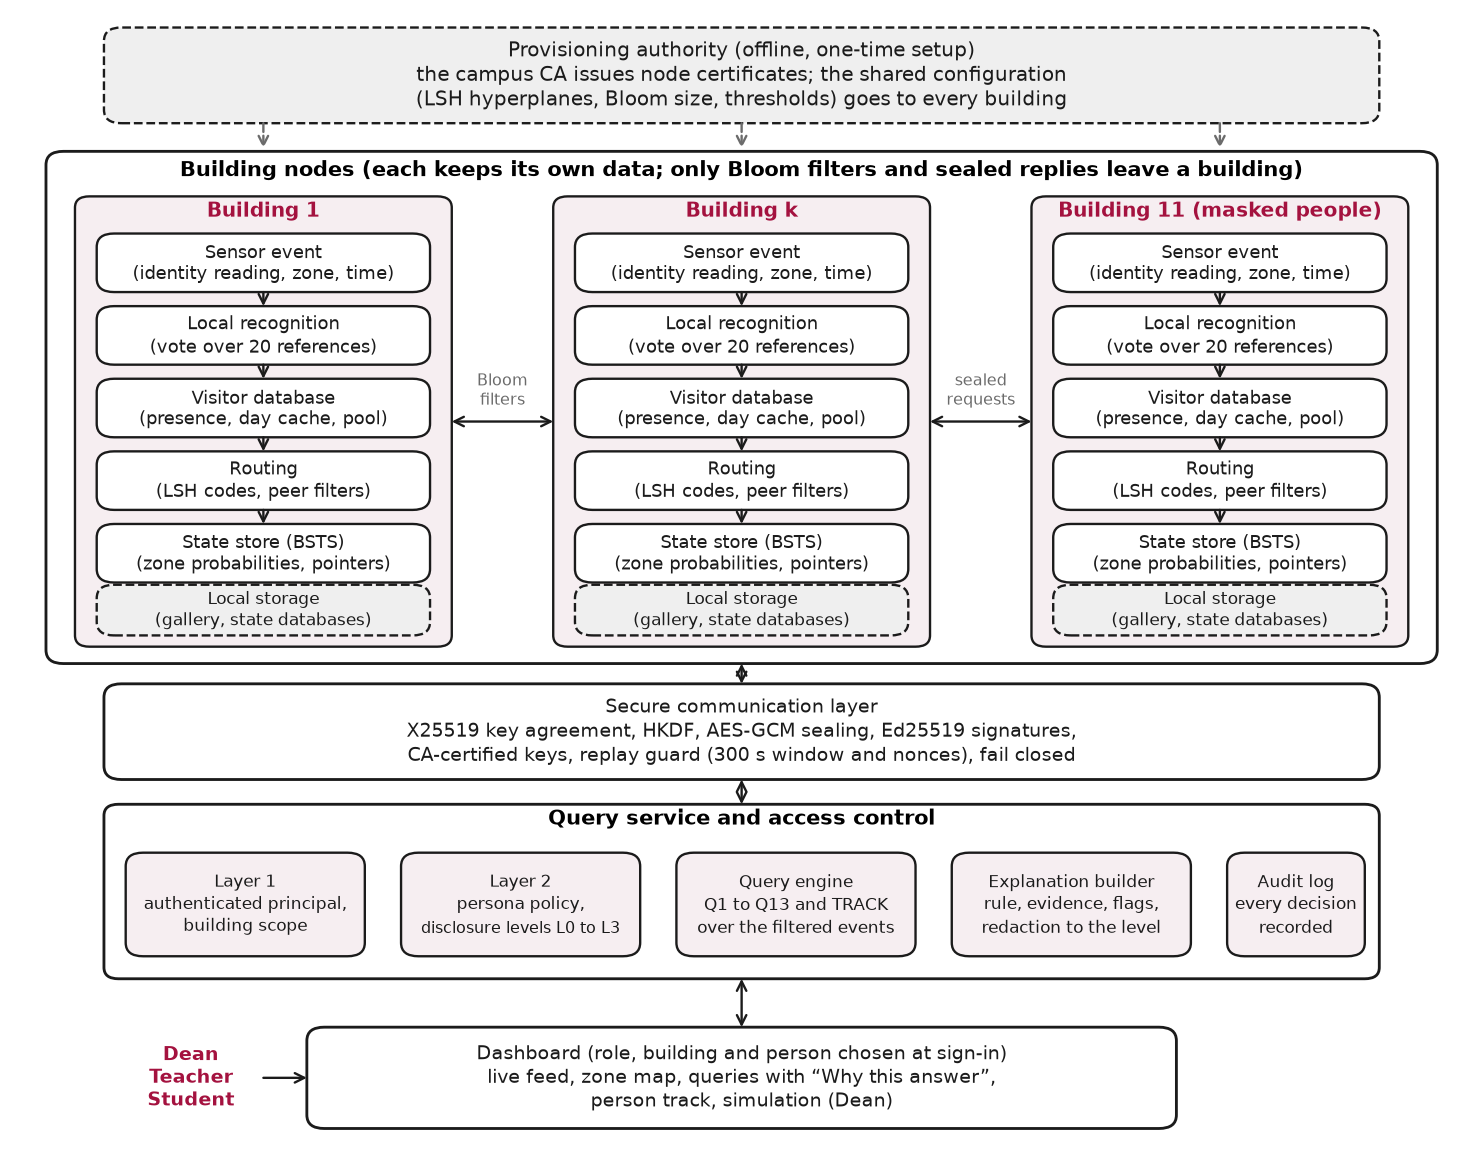
\includegraphics[width=0.78\textwidth]{figures/arch.png}
\caption{System architecture: building nodes, secure communication layer, access control layer and user interface}\label{fig:arch}
\end{figure}

\begin{figure}[htbp]
\centering
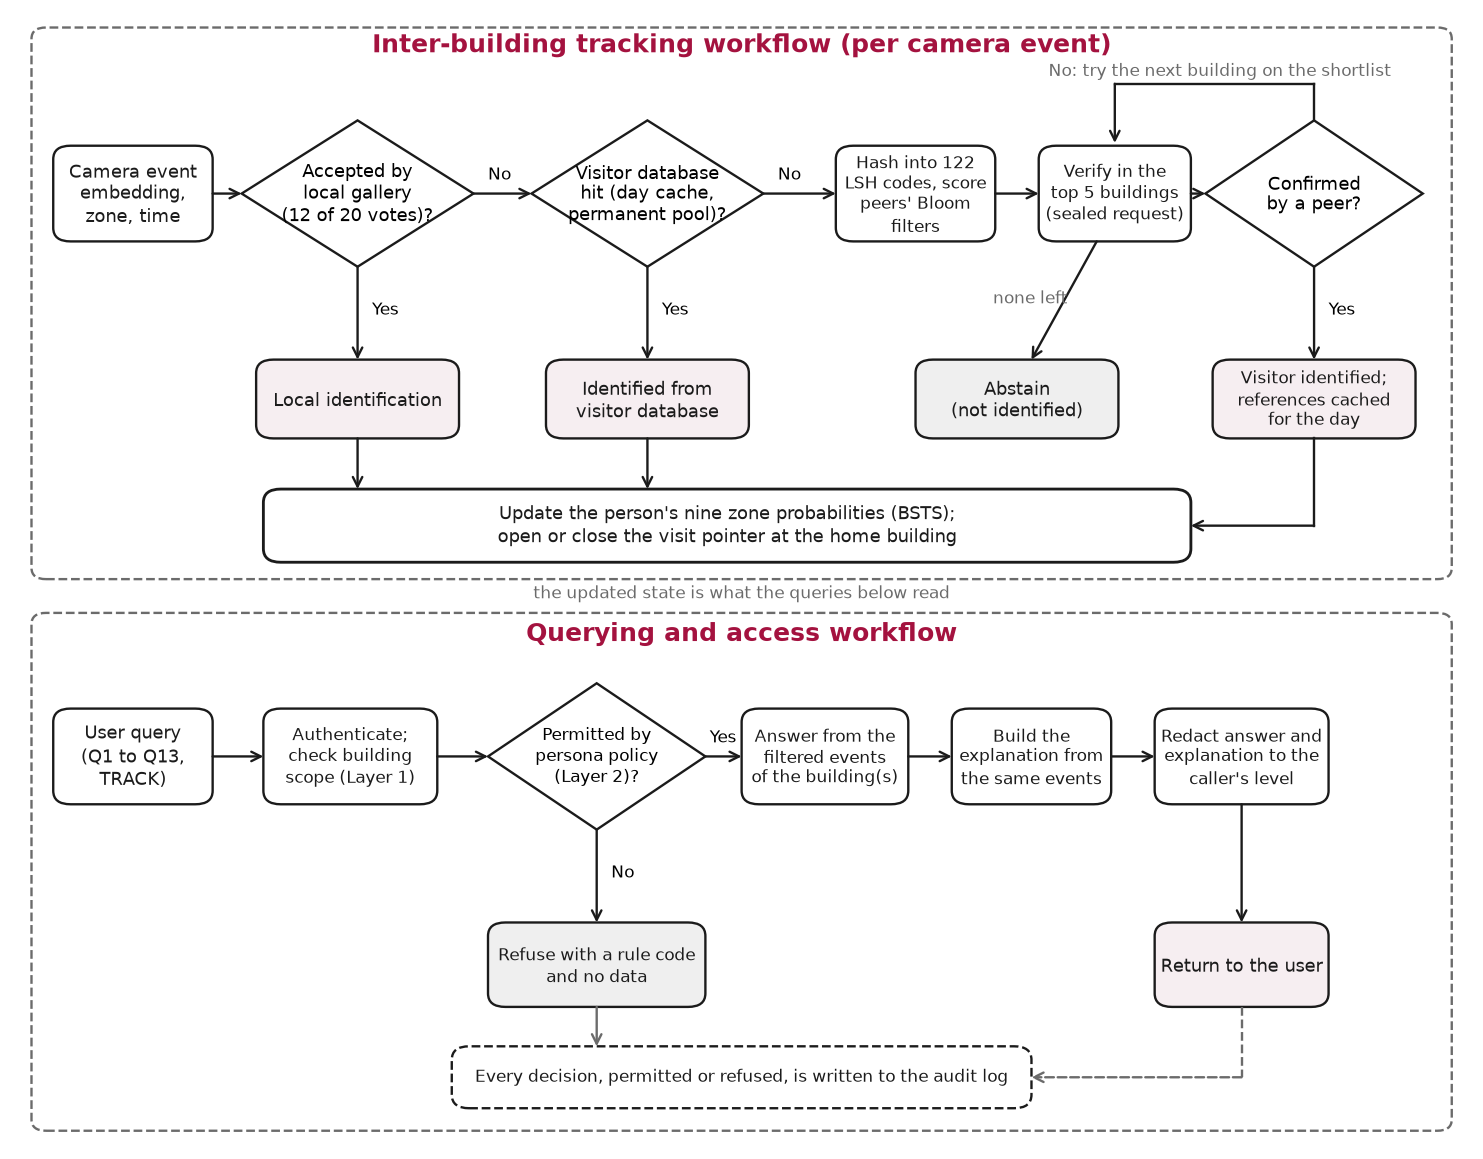
\includegraphics[width=0.85\textwidth]{figures/flow.png}
\caption{Inter-building tracking workflow and querying and access workflow}\label{fig:flow}
\end{figure}

Table~\ref{tab:stores} lists what each building keeps and what leaves it.



\begin{table}[htbp]
\centering
\caption{What a building keeps and what it shares}\label{tab:stores}
{\small\setlength{\tabcolsep}{4pt}\renewcommand{\arraystretch}{1.2}
\begin{tabular}{|p{3.6cm}|p{6.2cm}|p{4.8cm}|}\hline
\textbf{Item} & \textbf{Content} & \textbf{Leaves the building?}\\\hline
Gallery & 20 reference embeddings per registered occupant & Only the matched occupant's 20 references, sealed, after a confirmed match\\\hline
Bloom filter & Bit array of LSH items, 58,469 bits (7.3~KB), 7 hash positions, no ids or embeddings & Yes, published to all peers; one-way\\\hline
registered.db and visitor.db & Per-occupant zone probabilities and events, for own occupants and for visitors & No\\\hline
pointers.db & Visit pointers of own occupants who are away: occupant id, current building, entry and exit times & Read by location queries; contains no biometrics\\\hline
visitor\_\allowbreak pool.db and permanent\_\allowbreak visitors & Entry history and the embeddings of promoted frequent visitors & No\\\hline
Day cache & A visitor's 20 references, in memory for one simulated day & No; zeroed at day rollover\\\hline
\end{tabular}}
\end{table}


\section{Proposed approach and procedure}
\subsection{Embedding preprocessing and enrolment}
Faces are detected and aligned with SCRFD \cite{ref18} and embedded with an ArcFace model \cite{ref17} (512 dimensions). A raw embedding $e$ is normalised, centred with the mean $\bar{x}$ of the reference embeddings, and normalised again:
\begin{equation}
\hat{e}=\frac{e/\|e\|-\bar{x}}{\left\|\,e/\|e\|-\bar{x}\,\right\|}
\end{equation}
The $R=20$ preprocessed references of an occupant $u$ are averaged into a unit-norm centroid:
\begin{equation}
z_u=\frac{\sum_{r=1}^{R}\hat{e}_{u,r}}{\left\|\sum_{r=1}^{R}\hat{e}_{u,r}\right\|}
\end{equation}
The centroid is used only to build the Bloom filter. The 20 individual references are kept in the building for voting, because a centroid alone is a poor verifier.

\subsection{LSH codes and the Bloom filter}
Random hyperplanes (one Gaussian vector $w$ for each slot $l$ and bit $k$, drawn once and shared by all buildings) define $L=122$ slots of $K=11$ bits \cite{ref14}. The bit $h$ is the side of the hyperplane on which the embedding lies, and the $K$ bits of slot $l$ form an integer code $c_l$:
\begin{equation}
h_{l,k}(\hat{e})=\mathbf{1}\!\left[w_{l,k}^{\mathsf{T}}\hat{e}\geq 0\right],\qquad c_l=\sum_{k=0}^{K-1}h_{l,k}\,2^{k}
\end{equation}
Each occupant's centroid yields $L$ items, the item for slot $l$ being $l\cdot 2^{K}+c_l$, so a code counts as a match only in the same slot. The items of all occupants of a building are inserted into a Bloom filter \cite{ref12} with positions derived by double hashing \cite{ref16}. The filter is sized for 50 occupants at a target false-positive rate of 1\%, which gives 58,469 bits and 7 hash positions; with $50\times 122=6{,}100$ items the fill ratio is about 51\%. Only the packed bits and a few scalars are published (7.3~KB, or about 10~KB as a file): no ids, embeddings or centroids. Section~\ref{sec:res-bloom} measures how close the real false-positive rate is to the 1\% target.

\subsection{Local recognition, routing and verification}
A capture is first compared with the capturing building's own gallery. For every candidate occupant the angle between the capture and each of the 20 references is computed, and a reference votes if its angle is at most $80.43^{\circ}$. The winner is the occupant with most votes (ties broken by the smallest single angle); it is accepted only with at least $12$ votes. Figure~\ref{fig:flow} gives the flow and the listing below the steps.

If the local check does not accept, the capture is hashed in all $L$ slots. As well as the exact code, the $3$ least confident bits of each slot are flipped to give extra probes \cite{ref15}. Each peer's filter is tested; a building's score is the number of distinct slots that matched, on a 0 to $L$ scale, and the top $5$ buildings form the shortlist. They are contacted in rank order over the sealed channel and verify the capture with the same vote rule against their own occupants; the first confirmation ends the search. If no one confirms, the capture is not identified (abstain).

{\small
\begin{verbatim}
identify(capture q, building b):
  r = preprocess(q)
  (who, votes) = vote(own_gallery(b), r)          # >= 12 of 20 within 80.43
  if votes >= 12: return who                      # local occupant
  codes, margins = lsh_encode(r)                  # 122 slots of 11 bits
  score[c] = distinct slots of c's Bloom filter that match any probe
  for c in top_5(score):                          # best score first
      reply = sealed_request(c, r)                # only c sees the capture
      if reply.matched: return reply.occupant     # references come back sealed
  return None                                     # abstain
\end{verbatim}}

\subsection{Mask-occlusion handling}\label{sec:mask-handler}
The local recogniser contains a mask handler (module \texttt{recognition.mask\_\allowbreak handler}) that was part of the pipeline before this evaluation and is \emph{on by default}, so every result in Chapter~\ref{ch:results} includes its effect. After the first vote pass it measures the standard deviation of the per-occupant minimum reference angles over the building's gallery. If this spread exceeds 6.5$^{\circ}$ it treats the capture as suspected to be masked, loosens the acceptance angle by 4$^{\circ}$ (from 80.43$^{\circ}$ to 84.43$^{\circ}$), reduces the required votes by 25\% (from 12 to 9), repeats the vote and records a mask flag on the result.

The handler acts only on the \emph{local} check of the capturing building; the Bloom routing and the remote verification always use the plain thresholds. It is a statistical heuristic on the angle matrix, not an image classifier: a large spread means that one person stands out, which is the signature of a confident match rather than of a mask. Section~\ref{sec:res-mask} measures what it flags and what happens when it is switched off with \texttt{DSTS\_\allowbreak MASK\_\allowbreak HANDLER=off}.



\subsection{Tracking: probabilities and state}
For an identified event with candidate distances $d_i$ to each candidate occupant $i$, the occupant probabilities follow Definition 3.3 of the DSTS framework \cite{ref6}: with $\sigma$ the population standard deviation of the distances,
\begin{equation}\label{eq:prob}
p_i=\frac{\exp\!\left(-d_i^{2}/2\sigma^{2}\right)}{\sum_{l}\exp\!\left(-d_l^{2}/2\sigma^{2}\right)}
\end{equation}
The result is uniform over ties when $\sigma=0$. The Bloom score, vote counts and ground truth never enter this probability. The building state store keeps, for each occupant, a probability over the nine zones and updates it from each event. The zones are z1 Entrance, z2 Mail room, z3 Office, z4 Lounge, z5 Conference, z6 Classroom, z7 Cafeteria (reached only through the exit), z8 Exit, and zT, the transition zone to the outdoors; movement between buildings must pass through zT. The event is stored in the building that observed it: registered occupants in the registered database and visitors in the visitor database. The state is reset at the start of every simulated day.

\subsection{Dynamic visitor database and visit pointers}
A visitor is remembered in three layers (Table~\ref{tab:visitor}). A \emph{transition-zone rule} keeps a visitor who is waiting in zT out of other people's probability updates until they are seen outside zT. A \emph{visit pointer} (occupant id, current building, entry and exit times, no biometrics) is minted at the home building when the visitor arrives and closed at departure, so a location query follows the pointer instead of asking all buildings.

\begin{table}[htbp]
\centering
\caption{The three layers of the visitor database}\label{tab:visitor}
{\small\setlength{\tabcolsep}{4pt}\renewcommand{\arraystretch}{1.2}
\begin{tabular}{|p{2.8cm}|p{4.0cm}|p{3.8cm}|p{4.0cm}|}\hline
\textbf{Layer} & \textbf{Lifetime} & \textbf{Content} & \textbf{Used for}\\\hline
Presence & Memory, until the visitor leaves or the day ends & Who is inside and in which zone & Which rows the probability update covers\\\hline
Day cache & Memory, one simulated day; survives departure; zeroed at rollover & The visitor's 20 reference embeddings & Matching later captures the same day with no routing\\\hline
Entry history and permanent pool & Disk: visitor\_\allowbreak pool.db, permanent\_\allowbreak visitors & Every arrival; embeddings of frequent visitors & Recognising frequent visitors on any later day without routing\\\hline
\end{tabular}}
\end{table}

An arrival is the zT event of a visitor who is not inside. When a visitor's \emph{earlier} entries into a building already satisfy a rule from the configuration (default: three entries in seven days, or eight in thirty), the \emph{next} entry stores their embeddings permanently. From then on the visitor is matched from the permanent pool, on every day, without contacting any other building. A wrong identity stored in the cache persists for the rest of the day; such cases are counted separately in the results.

\subsection{Role-based access control}
Access control follows the role-based model of Sandhu et al. \cite{ref21}, extended with the relationship between the caller and the target. Every query passes two layers before execution. \emph{Layer~1} authenticates the principal and applies the building scope. \emph{Layer~2} is the persona policy, which returns a disclosure level for the pair (caller, target) and the purpose and time of the query. The levels are shown in Table~\ref{tab:levels} and the access model in Table~\ref{tab:access}. There are 1~Dean, 10~Teachers and 39~Students per building, and each Teacher has a class roster of about four students.

\begin{table}[htbp]
\centering
\caption{Disclosure levels}\label{tab:levels}
{\small\setlength{\tabcolsep}{4pt}\renewcommand{\arraystretch}{1.2}
\begin{tabular}{|p{1.2cm}|p{4.2cm}|p{9.2cm}|}\hline
\textbf{Level} & \textbf{Name} & \textbf{What the caller sees}\\\hline
L0 & None & Nothing; the request is refused with a reason code\\\hline
L1 & Presence & Availability only (defined in the policy; no current rule grants it)\\\hline
L2 & Current zone, coarse & Functional sector and the time rounded down to the hour\\\hline
L3 & Precise current & Exact zone, zone label, confidence and exact time\\\hline
L4 & Historical track & Full trajectory and dwell times\\\hline
\end{tabular}}
\end{table}

\begin{table}[htbp]
\centering
\caption{Access model (class-teacher RBAC)}\label{tab:access}
{\small\setlength{\tabcolsep}{4pt}\renewcommand{\arraystretch}{1.2}
\begin{tabular}{|p{2.6cm}|p{5.6cm}|p{3.0cm}|p{3.4cm}|}\hline
\textbf{Role} & \textbf{May follow} & \textbf{Disclosure} & \textbf{Cannot see}\\\hline
Dean (1 per building) & Teachers and students of their own campus (wherever they are), and the Deans of other buildings & L4 for both (rules RULE\_\allowbreak A\_\allowbreak OWN\_\allowbreak CAMPUS\_\allowbreak FULL and RULE\_\allowbreak A\_\allowbreak PEER\_\allowbreak DEAN\_\allowbreak TRACK) & Other campuses' teachers and students; visitors\\\hline
Teacher (10 per building) & Only the students on their class roster, in any building & L4 for roster students (RULE\_\allowbreak B\_\allowbreak ROSTER\_\allowbreak STUDENT) & Unassigned students, peer teachers, the Dean\\\hline
Student (39 per building) & Themselves in full; the teachers assigned to them & L4 for self, L3 for assigned teachers (RULE\_\allowbreak C\_\allowbreak ASSIGNED\_\allowbreak TEACHER) & Peer students, other teachers, the Dean\\\hline
\end{tabular}}
\end{table}

Building-level queries (Q1, Q2) return aggregates to everyone in their own building and the list of people only to a Dean; zone queries (Q10, Q12, Q13) filter each listed occupant through the same policy; students cannot run zone queries. There are fourteen query templates (Q1--Q14), covering occupancy, location, history, tracking and zone queries.

{\small\setlength{\tabcolsep}{4pt}\renewcommand{\arraystretch}{1.2}
}

\subsection{Explainable responses}
Each query builds an explanation from the same filtered event list that it used to compute the answer, never by recomputing afterwards. The explanation holds the decision rule in one sentence, the evidence events with their roles (decisive, last before $t$, carry-in state, zone visit), what was looked for and not found, uncertainty flags, what redaction withheld, and the visit pointer if one answered the query. Flags come from the identification provenance stored with every identified event (votes, routing rank, Bloom margin, whether the vote winner was also the nearest candidate) and are listed in Table~\ref{tab:flags}. The identity probability of Equation~\ref{eq:prob} is not used as a confidence signal because it is close to 1 for most misidentifications too. Before leaving the service the explanation is redacted to the caller's disclosure level, so it never shows more than the answer does.

\begin{table}[htbp]
\centering
\caption{Uncertainty flags}\label{tab:flags}
{\small\setlength{\tabcolsep}{4pt}\renewcommand{\arraystretch}{1.2}
\begin{tabular}{|p{4.6cm}|p{10.0cm}|}\hline
\textbf{Flag} & \textbf{Raised when}\\\hline
vote\_\allowbreak winner\_\allowbreak not\_\allowbreak nearest & The accepted occupant was not also the nearest candidate (strongest error signal)\\\hline
low\_\allowbreak votes & Fewer than 16 votes, although 12 suffice to accept\\\hline
verified\_\allowbreak by\_\allowbreak lower\_\allowbreak ranked\_\allowbreak building & The confirming building was not first on the shortlist\\\hline
narrow\_\allowbreak routing\_\allowbreak margin & The Bloom score gap between the top two buildings is below 5\\\hline
stale\_\allowbreak observation & A point-in-time answer rests on a sighting more than 60 minutes old\\\hline
pointer\_\allowbreak based & A value comes from a visit pointer with no identified sighting behind it\\\hline
\end{tabular}}
\end{table}

\subsection{Secure inter-building exchange}
Every message between buildings is sealed . The sender generates an ephemeral X25519 key \cite{ref23}, derives a symmetric key with HKDF-SHA256 \cite{ref22}, encrypts with AES-GCM \cite{ref25} using the whole header as associated data, and signs the header, nonce and ciphertext with Ed25519 \cite{ref24}. Replies are bound to their request. A campus certificate authority issues node certificates that bind both the signing key and the key-agreement key; expiry, revocation, subject and pinning are checked. A replay guard accepts a message only within a 300-second window and once per nonce, and runs after the signature check so the timestamp is authenticated. Any failed step yields no reply and nothing is admitted (fail closed).



\subsection{The masked building}
To study masked faces, 50 more people from RMFRD \cite{ref20} form an 11th building; each has 20 unmasked photos as the gallery and 20 masked probes (real photos topped up with augmented copies), embedded as for the other buildings and not shuffled by the seed (Appendix~\ref{app:setup}).

\subsection{Parameters}
Table~\ref{tab:params} lists the parameters used. The Bloom filter was configured for a 1\% false-positive rate, but Section~\ref{sec:res-bloom} shows that the effective rate that routing sees is about 3.5\% because LSH codes of different people collide.

\begin{table}[htbp]
\centering
\caption{Parameters used}\label{tab:params}
{\small\setlength{\tabcolsep}{4pt}\renewcommand{\arraystretch}{1.2}
\begin{tabular}{|p{7.4cm}|p{7.2cm}|}\hline
\textbf{Parameter} & \textbf{Value}\\\hline
LSH bits per slot $K$ / slots $L$ & 11 / 122\\\hline
Bloom target false-positive rate (configured) & 0.01\\\hline
Bloom effective false-positive rate (measured, Section~\ref{sec:res-bloom}) & about 3.5\%\\\hline
References per occupant $R$ & 20\\\hline
Accept angle / minimum votes & 80.43$^{\circ}$ / 12\\\hline
Shortlist size / extra probes & 5 / 3\\\hline
Mask handler (default on) & spread 6.5$^{\circ}$; +4$^{\circ}$; 25\% fewer votes\\\hline
Visitor promotion rule & 3 entries in 7 days or 8 entries in 30 days\\\hline
Uncertainty-flag thresholds & low votes below 16; narrow margin below 5; stale after 60 min\\\hline
\end{tabular}}
\end{table}

\subsection{API and dashboard}
The FastAPI server exposes login, query, tracking, occupancy and explanation endpoints; every data endpoint runs the same authentication, building scope and two-layer policy before it returns anything, and the dashboard is a static page that calls them. A simulation endpoint, open to Deans only, replays the run's recognised events against a simulated clock; a track endpoint returns one person's day, and a photo endpoint serves the captured or reference photo, both under the same policy.



\clearpage
\chapter{Results and Analysis}
\label{ch:results}
\section{Evaluation setup}
The evaluation uses 550 occupants in 11 buildings: the 500 CASIA-WebFace people dealt into 10 buildings of 50 by a seeded permutation, and the 50 masked people in building 11. One simulated day has 11,000 events, one for each of the 11,000 test photos; 8,800 are local (the person is in their home building) and 2,200 are visitor events. Every headline number in this chapter is the \emph{average over five random populations} (seeds 0 to 4); each seed places the same people in different buildings and draws a different event day. Where a single run is needed to show detail (the visitor outcome buckets, the mask-handler ablation and the screenshots), seed 42 is used and is named as such.



\textbf{Safeguards against bias.} Reference photos enrol people and are never events; test photos are events and are never enrolled. The mean face and the Bloom filters use reference photos only. The centralised baseline uses exactly the same preprocessing, thresholds and vote rule as the building nodes, so any difference is caused by routing and not by a stronger matcher. Ground truth is read only by the evaluation scripts; recognition, routing and tracking receive observable event fields only.

\section{Evaluation criteria}
All identification metrics use the one-vs-rest convention. An item has one true label and at most one predicted label out of $N_L$ labels. \textbf{TP}: the predicted label is the true label. \textbf{FP}: a wrong label was predicted. \textbf{FN}: the true label was not predicted (a wrong prediction or an abstention). \textbf{TN}: every other (item, label) pair, that is items $\times N_L-$TP$-$FP$-$FN. A wrong identity is therefore both an FP and an FN, and an abstention only an FN.
\begin{equation}
\mathrm{Precision}=\frac{TP}{TP+FP},\qquad \mathrm{Recall}=\frac{TP}{TP+FN},\qquad F_1=\frac{2PR}{P+R}
\end{equation}
Recall equals the share of events identified correctly, so it is also called identification accuracy. Because TN is in the millions, accuracy computed with TN is close to 1 and is not used to compare systems.

\textbf{Event level.} The label is the occupant id (550 labels), reported for all, local, visitor, masked and unmasked events. \textbf{State level.} State $s_k$ is the campus after event $k$; the label is (building, zone) with 99 labels, plus building (11 labels) and zone (9 labels) alone, and every occupant the system places counts, including visitors updated by other people's events. \textbf{Cost.} Gallery touched per lookup is the number of buildings whose gallery is searched divided by the number of buildings (the centralised server is 100\%); routing recall is the share of routed visitors whose home building is in the shortlist.

\textbf{Explanation criteria.} A flag is useful if it is carried by wrong answers and not by right ones. For identifications, \emph{share of wrong flagged} is the fraction of wrong identifications that carry at least one flag, and \emph{share of correct flagged} the false-alarm rate. For answers, an answer is wrong when it differs from the same query run over the identified events with their true occupants; flag \emph{precision} is the share of flagged answers that are wrong and \emph{recall} the share of wrong answers that are flagged. Overhead is the extra latency and response size of building the explanation. \textbf{Bloom criterion.} The effective false-positive rate is the share of the enrolled items of the other buildings that a building's filter reports as present.

\section{Result}
\subsection{Identification: decentralised against centralised}\label{sec:res-events}
Table~\ref{tab:central} compares the decentralised pipeline with the centralised search, and Table~\ref{tab:events} gives the confusion counts and scores, all averaged over the five seeds.

\begin{table}[htbp]
\centering
\caption{Identification accuracy and gallery touched (average of five seeds, 11,000 events per run)}\label{tab:central}
{\small\setlength{\tabcolsep}{4pt}\renewcommand{\arraystretch}{1.2}
\begin{tabular}{|p{3.2cm}|p{1.8cm}|p{2.6cm}|p{2.8cm}|p{1.8cm}|p{2.2cm}|}\hline
\textbf{Cohort} & \textbf{Events} & \textbf{Centralised accuracy} & \textbf{Decentralised accuracy} & \textbf{Gap (points)} & \textbf{Gallery touched}\\\hline
All events & 11,000 & 92.24\% & 91.54\% & 0.70 & 10.3\%\\\hline
Local & 8,800 & 91.98\% & 92.02\% & -0.04 & 9.1\%\\\hline
Visitor & 2,200 & 93.27\% & 89.61\% & 3.66 & 15.1\%\\\hline
Unmasked people & 10,000 & 95.48\% & 94.78\% & 0.70 & 10.1\%\\\hline
Masked people & 1,000 & 59.80\% & 59.06\% & 0.74 & 12.6\%\\\hline
\end{tabular}}
\end{table}



\begin{table}[htbp]
\centering
\caption{Event-level confusion counts and scores (average of five seeds; TN, in the millions, omitted)}\label{tab:events}
{\small\setlength{\tabcolsep}{4pt}\renewcommand{\arraystretch}{1.2}
\begin{tabular}{|p{3.0cm}|p{1.8cm}|p{1.5cm}|p{1.5cm}|p{2.0cm}|p{1.8cm}|p{1.6cm}|}\hline
\textbf{Cohort} & \textbf{TP} & \textbf{FP} & \textbf{FN} & \textbf{Precision} & \textbf{Recall} & \textbf{F1}\\\hline
All events & 10,069 & 245 & 931 & 0.976 & 0.915 & 0.945\\\hline
Local & 8,098 & 154 & 702 & 0.981 & 0.920 & 0.950\\\hline
Visitor & 1,971 & 91 & 229 & 0.956 & 0.896 & 0.925\\\hline
Unmasked & 9,478 & 173 & 522 & 0.982 & 0.948 & 0.965\\\hline
Masked & 591 & 72 & 409 & 0.892 & 0.591 & 0.711\\\hline
\end{tabular}}
\end{table}

Over all events the decentralised pipeline identifies 91.54\% against 92.24\% for the central search, a difference of 0.70 points, while each lookup touches 10.3\% of the galleries. Local events are marginally better with the pipeline (92.02\% against 91.98\%) because a person is matched only among the 50 people of their own building, so there are fewer look-alikes to confuse them with; the central search must discriminate among 550. The visitor events lose 3.7 points (89.61\% against 93.27\%), which is the cost of routing. The standard deviation over the five seeds is only 0.16 points (Section~\ref{sec:res-seeds}).

\subsection{Routing and the visitor database}\label{sec:res-visitors}
Table~\ref{tab:visitors} summarises how visitors are identified and the text below breaks one run (seed 42) down by outcome. In that run, of the 2,200 visitor events, 1,447 (about two thirds) are served from the building's visitor database (the same visitor sighted again the same day), 708 are routed, and the remaining 45 are visitors that an occupant of the capturing building wrongly accepted as a local person (a cross-population collision). The three groups add up to 2,200. Errors among the routed events are mostly routing misses that end in an abstention, and a smaller number of cases in which the right building is reached but the face still does not pass verification.

\begin{table}[htbp]
\centering
\caption{Visitor identification and tracking (average of five seeds)}\label{tab:visitors}
{\small\setlength{\tabcolsep}{4pt}\renewcommand{\arraystretch}{1.2}
\begin{tabular}{|p{8.4cm}|p{3.0cm}|}\hline
\textbf{Metric} & \textbf{Value}\\\hline
Visitor events per run & 2,200\\\hline
Precision / recall / F1 of visitor identification & 0.956 / 0.896 / 0.925\\\hline
Routing recall (home building in the top five) & 86.9\%\\\hline
Buildings contacted per routed lookup & 2.07\\\hline
Buildings contacted per visitor event, counting database hits & 0.67\\\hline
Visitor events served from the visitor database & 1,449 (about two thirds)\\\hline
Visit-pointer precision & 97.8\%\\\hline
Visitor recall in the tracked state: building / zone / building and zone & 0.945 / 0.924 / 0.891\\\hline
\end{tabular}}
\end{table}



The detailed run also shows how the headline gap should be read. The centralised search identified 92.24\% of its 11,000 events and the pipeline 91.76\%. The exact difference is 52 events out of 11,000, that is 0.47 points; the two rounded percentages differ by 0.48 only because of rounding. The five-seed gap in Table~\ref{tab:central} is 0.70 points.

\subsection{Stability across five random populations}\label{sec:res-seeds}
Table~\ref{tab:seeds} lists each of the five populations. The averages in this chapter are the means of these rows; the spread is small, so the detailed run is representative and does not depend on one lucky assignment of people to buildings. The visitor result varies most because it rests on fewer events.

\begin{table}[htbp]
\centering
\caption{Results per random population (11,000 events each)}\label{tab:seeds}
{\small\setlength{\tabcolsep}{4pt}\renewcommand{\arraystretch}{1.2}
\begin{tabular}{|p{1.6cm}|p{2.2cm}|p{2.2cm}|p{2.2cm}|p{2.4cm}|p{2.2cm}|}\hline
\textbf{Seed} & \textbf{Accuracy, all} & \textbf{Local} & \textbf{Visitor} & \textbf{Routing recall} & \textbf{Masked recall}\\\hline
0 & 91.76\% & 92.11\% & 90.36\% & 87.1\% & 59.4\%\\\hline
1 & 91.35\% & 91.75\% & 89.73\% & 87.0\% & 59.3\%\\\hline
2 & 91.62\% & 92.08\% & 89.77\% & 86.4\% & 58.9\%\\\hline
3 & 91.44\% & 91.97\% & 89.32\% & 87.1\% & 59.1\%\\\hline
4 & 91.52\% & 92.18\% & 88.86\% & 86.6\% & 58.6\%\\\hline
\textbf{Mean} & 91.54\% & 92.02\% & 89.61\% & 86.9\% & 59.1\%\\\hline
95\% CI ($\pm$ points) & 0.20 & 0.21 & 0.69 & 0.4 & 0.4\\\hline
\end{tabular}}
\end{table}

\subsection{Tracking state against the state ground truth}\label{sec:res-state}
Table~\ref{tab:state} reports the state-level scores. After every one of the 11,000 events the whole campus state, that is who is in which building and zone, is compared with the true state recorded by the simulation, and the scores are averaged over the 11,000 states of a run and then over the five seeds.

\begin{table}[htbp]
\centering
\caption{State-level scores against the state ground truth (average of five seeds)}\label{tab:state}
{\small\setlength{\tabcolsep}{4pt}\renewcommand{\arraystretch}{1.2}
\begin{tabular}{|p{3.4cm}|p{1.8cm}|p{2.4cm}|p{2.0cm}|p{1.6cm}|p{2.6cm}|}\hline
\textbf{Level} & \textbf{Labels} & \textbf{Precision} & \textbf{Recall} & \textbf{F1} & \textbf{Visitor recall}\\\hline
Building & 11 & 0.956 & 0.944 & 0.950 & 0.945\\\hline
Zone & 9 & 0.921 & 0.910 & 0.916 & 0.924\\\hline
Building and zone & 99 & 0.901 & 0.890 & 0.896 & 0.891\\\hline
\end{tabular}}
\end{table}



Building-level state, that is knowing which building each person is in after every event, reaches an F1 of 0.950; the zone within a building and the combination are harder because the nine-zone belief is updated from one event at a time. The standard deviation of the building-level F1 over the five seeds is 0.0040.

\subsection{Masked people}\label{sec:res-masked}
Table~\ref{tab:events} (rows Masked and Unmasked) compares the 50 masked people of building 11 (1,000 events per run) with everyone else (10,000 events). Masked people are identified 59.1\% of the time against 94.8\% for unmasked people. When the system does answer for a masked person it is right 89.2\% of the time, so the loss is mostly missed identifications rather than wrong ones. A masked probe is about 72$^{\circ}$ from its own unmasked gallery on average, close to its nearest other person (about 74$^{\circ}$), so the gallery gives little margin. Routing is also weaker for masked visitors: the right building is found less often and ranked lower.





\subsection{What was tried for masked faces, and the mask handler}\label{sec:res-mask}
Three ideas for improving masked recognition were tested offline on the 1,000 masked probes against the 50-person gallery, using the real thresholds (80.43$^{\circ}$ and 12 votes): adding ten synthetic-masked templates per person to the gallery; matching on the upper face only, by blanking the lower part of both gallery and probe; and relaxing the accept angle and votes when a mask is suspected. Each mostly traded abstentions for wrong answers (best case: 66.1\% correct but 16.9\% wrong, against 59.8\% correct and 7.0\% wrong now). Relaxing the thresholds alone raised wrong identities from 7.0\% to 28.4\% and let strangers (people of other buildings) be accepted 31\% of the time. F1 stayed at 0.72 or fell. Without any threshold, the nearest person is the right one only 65--70\% of the time whatever the gallery, so the limit is the face model, which was not trained for masks, and the noisy web labels. Enrolling five to eight \emph{real} masked photos per person, held out from the probes, gave about five points more in rank-1 accuracy.







\textbf{The existing mask handler.} The handler described in Section~\ref{sec:mask-handler} flags a probe as masked when the spread of per-person minimum angles is large. Measured on the detailed run it flags none of the 850 masked local events and 3,355 of the 7,950 unmasked local events (42\%), because a large spread means that one person stands out, not that a mask is present. With the handler switched off (\texttt{DSTS\_\allowbreak MASK\_\allowbreak HANDLER=off}) on the same events, masked results are unchanged (590 TP, 70 FP) and unmasked people gain 21 correct identifications (9,525 against 9,504) and lose 22 false accepts (125 against 147). The default is left on, so all other results include this small effect, and the finding is reported as a limitation.

\subsection{Explanation quality}\label{sec:res-expl}
Explanation quality was measured in three ways: whether explanations are faithful to the answers, whether the uncertainty flags catch real errors, and what the explanations cost. All numbers below are averages over the five seeds and were produced on the current system (11 buildings, the masked building included) by \texttt{evaluation.evaluate\_\allowbreak explanations}.

\textbf{Faithfulness and leakage.} Every explanation is built from the events that produced the answer. For each query class, tests with a yes, a no and an empty answer (40 cases) check that every evidence item is one of the engine's own events and that the answer recomputed from the evidence equals the engine's answer. Further tests check that no explanation reveals more than its answer at any disclosure level, that routing details are hidden below L4, and that cached explanations are never shared across levels. All pass (Section~\ref{sec:res-security}).

\textbf{Do the flags catch errors?} Table~\ref{tab:expl-id} scores the identification flags against the ground truth. On average 10,314 events per run are identified, of which 245 are wrong. 74.2\% of the wrong identifications carry at least one flag, and 3.8\% of the correct ones do (the false-alarm rate); of all flagged events 32.3\% are wrong. The flags work best on routed visitors (87\% of wrong ones flagged) and on local identifications (74\%). They almost never flag a wrong identification that comes from the visitor database (3\%), because that path re-matches against cached references and carries little provenance; these are the errors that persist for the rest of a day, and are the main weakness of the explanation layer. The strongest single flag is \texttt{vote\_\allowbreak winner\_\allowbreak not\_\allowbreak nearest}: 66\% of the identifications carrying it are wrong.

\begin{table}[htbp]
\centering
\caption{Uncertainty flags on identifications (average of five seeds)}\label{tab:expl-id}
{\small\setlength{\tabcolsep}{4pt}\renewcommand{\arraystretch}{1.2}
\begin{tabular}{|p{4.4cm}|p{1.8cm}|p{1.8cm}|p{2.4cm}|p{2.4cm}|p{1.8cm}|}\hline
\textbf{Group} & \textbf{Identified} & \textbf{Wrong} & \textbf{Wrong, flagged} & \textbf{Correct, flagged} & \textbf{Flagged that are wrong}\\\hline
All identified events & 10,314 & 245 & 74.2\% & 3.8\% & 32.3\%\\\hline
Local & 8,259 & 161 & 73.7\% & 2.4\% & 38.0\%\\\hline
Routed visitors & 613 & 72 & 86.8\% & 34.6\% & 25.1\%\\\hline
Visitor database & 1,442 & 12 & 2.8\% & 0.01\% & 67\%\\\hline
\end{tabular}}
\end{table}



At the level of answers, the flags are scored over a grid of real queries (Q6 at every hour, Q7 over four two-hour windows and TRACK, for every identified occupant). On average 7,589 answers per run were scored; 24.6\% carry a flag; 912 are wrong, of which 80.2\% are flagged (recall) and 39.2\% of the flagged answers are wrong (precision). A flag is therefore a good reason to look twice, not a verdict: most flagged answers are still right, but four of every five wrong answers are flagged.



\textbf{What do explanations cost?} Each query type was run 100 times per seed with explanations off and on. Summed over all fourteen queries the latency rises from 16.3~ms to 17.4~ms, an increase of 8.0\%. The aggregate queries (Q1, Q13) cost most because they gather one evidence item per person; the point queries cost almost nothing. The response grows more than the latency: with the full L4 explanation, the sum of the response sizes rises from about 15,820 to 117,290 bytes, because the evidence is listed. Lower disclosure levels receive much less.





An earlier measurement on the 10-building system, before the masked building existed, found a higher flag recall (84\% against 74\% here). The difference is the cohort: for unmasked people 80.6\% of wrong identifications are flagged and 2.3\% of correct ones, close to the earlier figures, but for masked people only 58.7\% of wrong identifications are flagged while 27.5\% of correct ones are flagged too, because masked captures have low votes and narrow margins.

\subsection{The Bloom filters' real false-positive rate}\label{sec:res-bloom}
Each filter is sized for a 1\% false-positive rate on the assumption that its items behave like independent random keys. LSH codes of different people are not independent: two occupants whose embeddings fall on the same side of the same hyperplanes receive the same code in that slot. The effective rate was therefore measured directly, by testing the enrolled items of the ten other buildings against each building's filter and averaging over the buildings and the five seeds.





The effective rate is about 3.5 times the configured one. The Bloom array itself is not at fault: random integers that were never inserted are reported at 0.95\%, essentially the 1\% target. The excess comes from the codes: 2.63\% of the items of other buildings already equal an enrolled item in the same slot, close to the 2.44\% expected if the codes of 50 occupants were spread evenly over 2048 values. This is the same finding as in the earlier routing study \cite{ref28}, which measured $3.54\pm0.02\%$ on 10 buildings; the five-seed value here, measured on 11 buildings, is 3.55\%.

\textbf{Privacy consequence.} The filter is one-way, but membership in it can be tested, and a positive does not prove that a particular face is enrolled in the building: with an effective rate of about 3.5\% on top of genuine matches, a positive is ambiguous. That ambiguity is useful, and it is why routing only ranks buildings and never identifies anyone; identification needs the exact vote on the real references in the shortlisted buildings. The same finding also means that the configured 1\% must not be quoted as the system's false-positive rate, and that the privacy argument should rest on the one-way encoding and on the verification step, not on a small false-positive rate. No formal privacy guarantee is claimed.

\subsection{Verification of the security and policy layers}\label{sec:res-security}
The security, policy and explanation layers are verified by 575 automated tests (Table~\ref{tab:tests}). They include attack cases written for this project: tampering with every header field of a sealed message, replay, wrong sender or recipient, a revoked certificate, brute-force login, a token used as another person, and cache sharing across roles.

\begin{table}[htbp]
\centering
\caption{Automated tests by area}\label{tab:tests}
{\small\setlength{\tabcolsep}{4pt}\renewcommand{\arraystretch}{1.2}
\begin{tabular}{|p{4.6cm}|p{1.4cm}|p{8.6cm}|}\hline
\textbf{Area} & \textbf{Tests} & \textbf{What is checked}\\\hline
access\_\allowbreak control & 112 & Every policy cell, structured Layer-1 decisions, building scope, lockout, credentials, tickets, API-level RBAC attacks\\\hline
secure\_\allowbreak transfer & 61 & Sealed payloads: tampering, replay, wrong sender or recipient, revoked certificate, fail closed, strict decoding\\\hline
api & 96 & Login and demo sign-in, queries per role, caching, zone and time-frame views, simulation control, person track and photos, dashboard adapter\\\hline
queries & 184 & Query engine, multi-day normalisation, explanation faithfulness, leakage and uncertainty, CLI access rules\\\hline
pipeline, population, events, evaluation & 98 & Phase 2, 3 and 4, visitor database, seeded populations, event generation, ground truth, confusion metrics\\\hline
standalone, centralised, state library & 19 & Standalone demo, centralised baseline, state library\\\hline
shared utilities & 5 & Dated timestamps, time-window arithmetic\\\hline
\textbf{Total} & \textbf{575} & All passing on the final commit\\\hline
\end{tabular}}
\end{table}

A persona matrix tool replays 64 requests (Dean, Teacher, Student and an outsider against each query type and target type) and checks the decision, the rule code and the disclosure level of each. A request for a person in another building is denied unless a relationship allows it: a Teacher may follow a rostered student wherever the student is, and a Dean may follow the Deans of other buildings; every other cross-building request is refused with a rule code such as \texttt{RULE\_\allowbreak C\_\allowbreak CROSS\_\allowbreak BUILDING\_\allowbreak DENIED} or \texttt{RULE\_\allowbreak A\_\allowbreak CROSS\_\allowbreak BUILDING\_\allowbreak B\_\allowbreak C\_\allowbreak DENIED}.



\subsection{The dashboard}\label{sec:res-ui}
The dashboard is a demonstration of the access model as much as of the tracking. A Dean starts a simulation of one day, one week or one month: the recognised events of the run are replayed against a simulated clock, and the campus map, the occupancy, the live feed and every query follow it (Figure~\ref{fig:ui-overview}). Later days replay each person's recorded events with the times shifted by up to ten minutes, and weekends are quieter; no identity, building or zone is invented. The person at the keyboard is chosen by role, building and name (any Dean, Teacher or Student of any building), and what the page shows is then decided only by the two policy layers: the same feed shows a Dean of building 8 every event of that campus, a Teacher only the assigned students, and a Student only themselves.

Choosing a building shows its nine zones; choosing a zone lists who was there in the time frame, named only where the role may see the exact location. Choosing a person opens their day as a track across buildings and zones (Figure~\ref{fig:ui-track}): each photo is the one the camera captured at that moment, a blue dashed line joins sightings inside a building and a red one a move to another building. The track and the photos are shown only where the role may see the exact location (disclosure L3 or higher), so a Student cannot follow a Dean. A query returns its answer with the ``Why this answer'' card (Figure~\ref{fig:ui-dean}).

\begin{figure}[htbp]
\centering
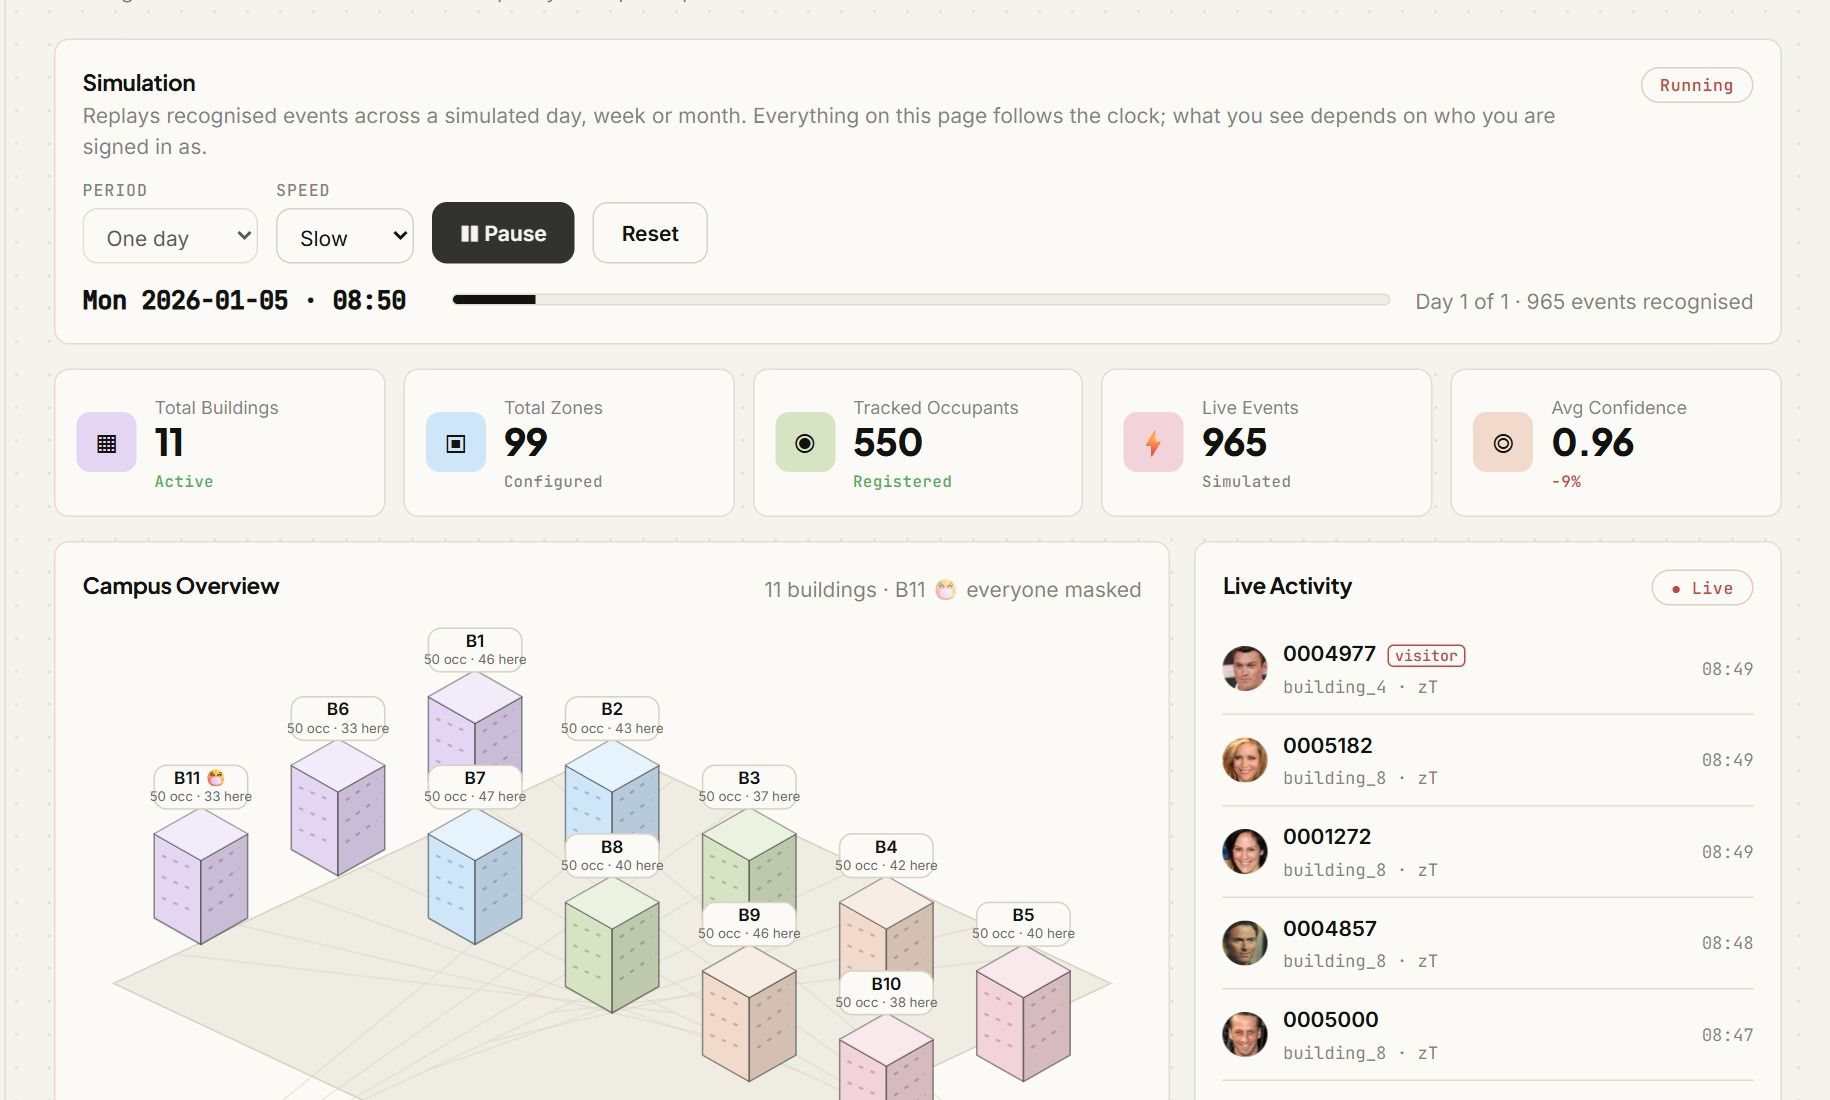
\includegraphics[width=0.58\textwidth]{figures/ui_overview.png}
\caption{Overview with a simulation running: clock, progress, counts and a live feed with photos; the sign-in (role, building, person) is at the top right}\label{fig:ui-overview}
\end{figure}

\begin{figure}[htbp]
\centering
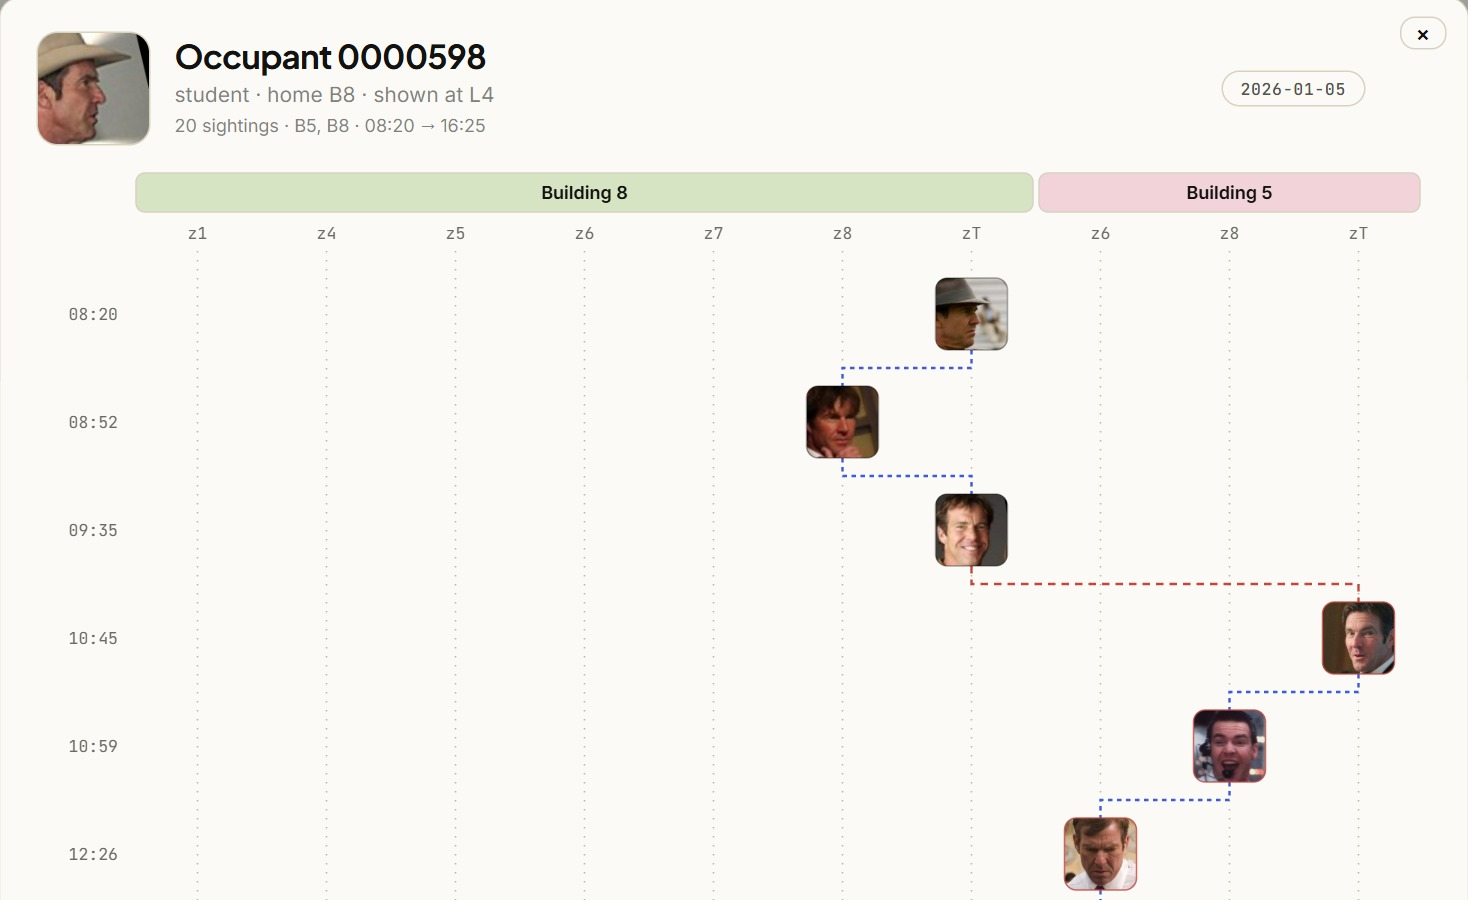
\includegraphics[width=0.5\textwidth]{figures/ui_track.png}
\caption{The track of one person across two buildings, with the photo captured at each sighting}\label{fig:ui-track}
\end{figure}

\begin{figure}[htbp]
\centering
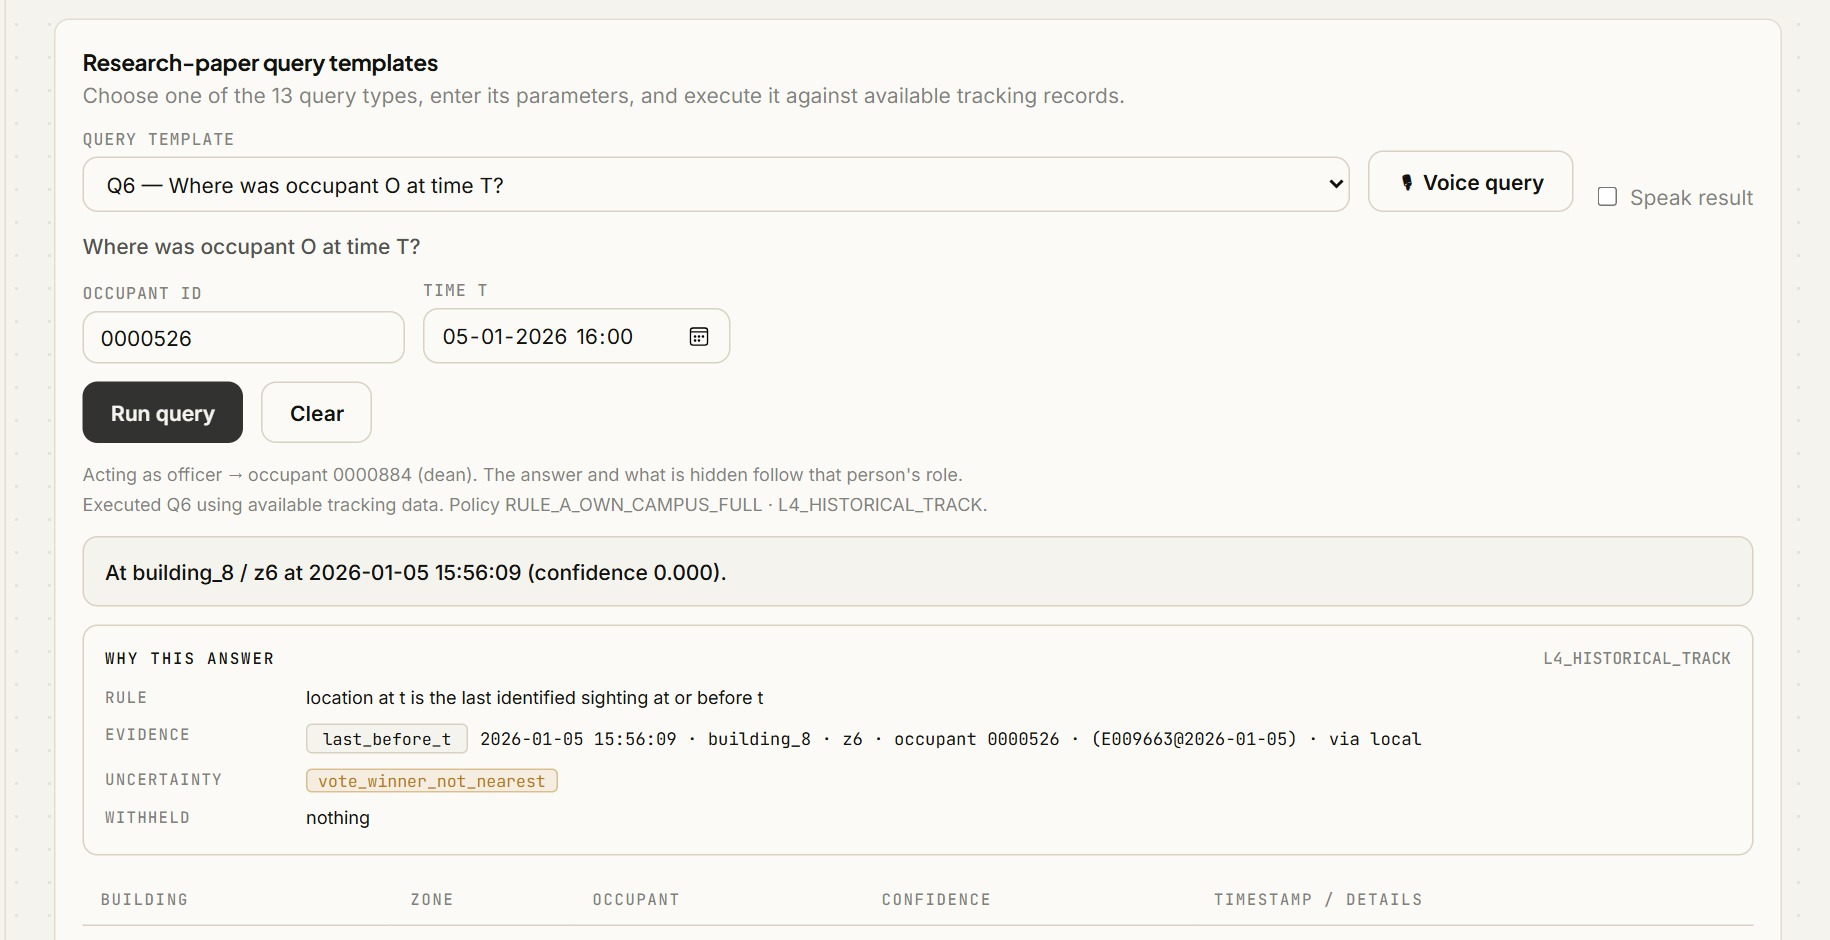
\includegraphics[width=0.58\textwidth]{figures/ui_query_dean.png}
\caption{A Dean's query with its ``Why this answer'' card (rule, evidence, uncertainty, withheld)}\label{fig:ui-dean}
\end{figure}

\section{Comparative Analysis}
Table~\ref{tab:comparison} compares the approaches. The fair comparison for this project is the same pipeline with a central search; other published systems \cite{ref1,ref2,ref3,ref4,ref5} use different data and tasks and cannot be compared number for number.

\begin{table}[htbp]
\centering
\caption{Comparison with the baseline and the approaches in the literature}\label{tab:comparison}
{\small\setlength{\tabcolsep}{4pt}\renewcommand{\arraystretch}{1.2}
\begin{tabular}{|p{4.0cm}|p{3.2cm}|p{4.2cm}|p{3.2cm}|}\hline
\textbf{Approach} & \textbf{Visitor lookup} & \textbf{Face data leaving a building} & \textbf{Result here}\\\hline
Centralised search over all galleries (baseline) & One global search & Galleries pooled in one store & 92.24\%; 100\% of the gallery searched\\\hline
Decentralised LSH + Bloom routing (this work) & Rank by Bloom score, verify top 5 & Only a 7.3~KB Bloom filter; references move only after a confirmed match & 91.54\%; 10.3\% of the gallery\\\hline
DSTS base paper \cite{ref6} & Central master list & Master list of visitor embeddings & Not re-run; replaced by the row above\\\hline
Edge-camera tracking \cite{ref1,ref2,ref3,ref4,ref5} & Within one site & Not applicable & No cross-building identity, RBAC or explanations\\\hline
\end{tabular}}
\end{table}

Routing costs 0.70 points overall and 3.7 points on visitors, in exchange for touching about a tenth of the gallery and never pooling it.

\textbf{Relation to the earlier routing study.} The manuscript on routing alone \cite{ref28} reports 92.81\% correct identification for the decentralised policy that verifies all five shortlisted buildings against 95.50\% for the centralised search. Those numbers measure something different and should not be compared directly: the earlier study counts \emph{routed visitor events only}, uses 10 buildings and 20 seeds, and compares against a central search over the 450 identities outside the capturing building. This report counts \emph{all} 11,000 events, uses 11 buildings including the masked building, counts visitors served from the visitor database as identified, and averages five seeds. The visitor accuracy here (89.6\%) is lower mainly because masked visitors are included, and the central search (92.2\%) is lower because it separates 550 identities instead of 450.

\section{Discussion and Interpretation}
The results meet the objectives that can be measured. Decentralised identification is within 0.7 points of a central search overall while touching about 10\% of the galleries, so the privacy and locality gain costs little accuracy (objectives 1 and 4). Most visitor events are cheap because repeat sightings the same day come from the day cache, which is why the number of buildings contacted per visitor event is well below one. Tracking is reliable at building level and good at zone level (objective 1).

The access model and the explanations are verified by tests, flag scores and a persona matrix (objectives 2, 3 and 5). The flags catch about three quarters of the wrong identifications for about eight per cent of extra latency, but the visitor database, whose errors are rarely flagged, is the weak spot.

Two findings change how the system should be described. First, the Bloom filters' real false-positive rate is about 3.5\%, not the 1\% configured, because LSH codes collide; routing remains useful because verification is exact, but the privacy argument must not rely on the small configured rate. Second, masked identification is limited by the face model and not by the routing design, and the mask handler that was meant to help does not do so: it never fires for masked people and slightly harms unmasked ones.

\section{Limitations}
\begin{itemize}
\item The network, cameras and the face detector are simulated. Arrays are plaintext in memory before sealing and after opening, and the certificate authority is a stand-in whose signature is a message authentication code, not a real public-key infrastructure.
\item The API has no TLS unless a reverse proxy adds it, no browser security headers, and no encryption of the stored embeddings and state databases. No outside penetration test or fuzzing was done; the attack tests are those the team wrote.
\item Token secrets, caches and lockout counters are per process, so they would not hold across several servers; the dashboard's demo mode lets any viewer act as any role by design.
\item The masked building uses web-crawled photos with some wrong labels, and 20\% of the masked probes are augmented copies. Masked results are not an accuracy estimate for new people.
\item A wrong identity stored in the visitor cache stays for the rest of that day, is rarely flagged, and a visitor whose departure is not identified stays ``present'' until the day ends.
\item The effective Bloom false-positive rate (about 3.5\%) is higher than configured, and no formal privacy guarantee is claimed.
\item Every visitor is a person registered in some building; people who are registered nowhere cannot be identified and are left unidentified.
\item Only 550 people in 11 buildings were measured; larger scale is untested. The same 20 test photos per person are reused across days in multi-day runs.
\item Results come from simulated movement on replayed photos, not from live video.
\end{itemize}

\clearpage
\chapter{Conclusion}
\section{Conclusion}
This project built and evaluated a system that identifies and tracks occupants across buildings without pooling face data, answers queries according to the caller's role and relationship, and explains each answer. A visitor is found by routing a capture with LSH codes and per-building Bloom filters and verifying it only in the shortlisted buildings. On 11,000 events per day, averaged over five random populations, it identifies 91.5\% correctly against 92.2\% for a centralised search, touching 10.3\% of the galleries; the 95\% confidence interval of the accuracy is $\pm0.20$ points, and building-level state F1 is 0.950. A dynamic visitor database makes about two thirds of the visitor events free of routing. A two-layer class-teacher policy, sealed transfers and redacted explanations are implemented and covered by 575 automated tests. The uncertainty flags attached to answers catch about three quarters of the wrong identifications and four in five wrong answers for about 8\% of extra latency, although they rarely flag errors that come from the visitor database. Masked people are the hard case at 59.1\%, and the evidence points to the face model, not the routing, as the limit. Measuring the Bloom filters showed that their effective false-positive rate is about 3.5\%, not the 1\% configured, so the privacy argument rests on the one-way encoding and on exact verification. All six objectives are achieved in simulation (Table~\ref{tab:status}); the security work is a tested design on a simulated network and not a hardened deployment.

\begin{table}[htbp]
\centering
\caption{Objective-wise status}\label{tab:status}
{\small\setlength{\tabcolsep}{4pt}\renewcommand{\arraystretch}{1.2}
\begin{tabular}{|p{4.6cm}|p{2.0cm}|p{2.6cm}|p{5.2cm}|}\hline
\textbf{Objective} & \textbf{Planned} & \textbf{Status} & \textbf{Evidence}\\\hline
1. Multi-building DSTS extension & Mid review & Achieved & BSTS over 11 buildings; building-level state F1 0.950\\\hline
2. RBAC query interface & 24/9/26 & Achieved & Two layers, class-teacher model, every policy cell tested, 64-request persona matrix\\\hline
3. Explainable responses & 26/9/26 & Achieved & Faithfulness cases, flag recall 74\% on identifications, 8\% overhead\\\hline
4. LSH + Bloom routing & Mid review & Achieved & 10.3\% of gallery touched, 0.7-point accuracy cost; effective false-positive rate 3.5\%\\\hline
5. Security layer & 2/10/26 & Achieved (simulated network) & Sealed transfers, tokens, lockout, audit log\\\hline
6. Evaluation & Final review & Achieved & Event and state TP/FP/FN/TN, five seeds, centralised baseline, explanation and Bloom measurements\\\hline
\end{tabular}}
\end{table}

\section{Future work}
Two directions follow directly from the results.

\textbf{Better masked recognition.} Masked people are identified only 59\% of the time. The next steps are a face model trained with masks instead of one trained on unmasked faces; a real mask detector, because the existing angle-spread heuristic flags the wrong people; enrolling a few real masked photos per person, which gave about five points of rank-1 accuracy in the offline tests; and using tracking context, such as who is already inside the building, to reduce masked errors. Each can be validated on the same seeds and the same masked building, with the masked F1 of Table~\ref{tab:events} as the target and the unmasked F1 as a check that nothing else gets worse.

\textbf{Unknown visitor re-identification.} Today a visitor must be registered in some building, and a face that nobody knows is left unidentified. A future version should re-identify unknown visitors across buildings and days: keep one-way codes of the unknown faces (LSH with Bloom filters) under a temporary identifier, link their sightings into a track, and let an administrator later name or purge them. This needs retention and privacy rules, and a check that two different strangers are not merged, which can be measured with the same precision and recall used here once unregistered people are added to the simulated population.

\clearpage
\renewcommand{\bibname}{References}

\begin{thebibliography}{99}
\phantomsection
\addcontentsline{toc}{chapter}{References}

\setlength{\itemsep}{6pt}
\setlength{\parskip}{0pt}

% Journal paper format
\bibitem{ref1}
C. Hegde \textit{et al.},
``Indoor group identification and localization using privacy-preserving edge computing distributed camera network,''
\textit{IEEE J. Indoor Seamless Position. Navig.},
vol. 2, pp. 51--60,
2024, doi: 10.1109/JISPIN.2024.3354248.

\bibitem{ref2}
H. Kwon \textit{et al.},
``A feasibility study on indoor localization and multiperson tracking using sparsely distributed camera network with edge computing,''
\textit{IEEE J. Indoor Seamless Position. Navig.},
2023, doi: 10.1109/JISPIN.2023.3337189.

% Journal paper with an article number instead of page numbers
\bibitem{ref3}
S. Yang, F. Ding, P. Li, and S. Hu,
``Distributed multi-camera multi-target association for real-time tracking,''
\textit{Sci. Rep.},
vol. 12,
Art. no. 11052, 2022,
doi: 10.1038/s41598-022-15000-4.

\bibitem{ref4}
S. Casao, A. Naya, A. C. Murillo, and E. Montijano,
``Distributed multi-target tracking in camera networks,''
arXiv:2010.13701, 2021.

\bibitem{ref5}
B. Gaikwad and A. Karmakar,
``Smart surveillance system for real-time multi-person multi-camera tracking at the edge,''
\textit{J. Real-Time Image Process.},
2021, doi: 10.1007/s11554-020-01066-8.

\bibitem{ref6}
L. Mohan and V. Menon,
``Modelling large scale camera networks for identification and tracking: an abstract framework,''
\textit{IET Comput. Vis.},
vol. 14, no. 7, pp. 426--433,
2020.

\bibitem{ref7}
V. Menon, B. Jayaraman, and V. Govindaraju,
``The three Rs of cyberphysical spaces,''
\textit{Computer},
vol. 44, no. 9, pp. 73--79,
2011.

\bibitem{ref8}
S. P. Nair, K. A. Reddy, P. K. Alluri, and S. Lalitha,
``Face recognition and tracking for security surveillance,''
\textit{J. Intell. Fuzzy Syst.},
vol. 41, no. 5, pp. 5337--5345,
2021, doi: 10.3233/JIFS-189856.

\bibitem{ref9}
Z. Wu \textit{et al.},
``Learning-based tracking-before-detect for unconstrained indoor human tracking using RF signal,''
\textit{IEEE Trans. Mobile Comput.},
vol. 24, no. 6, pp. 4777--4793,
2025, doi: 10.1109/TMC.2025.3529501.

\bibitem{ref10}
C. Rathgeb, F. Breitinger, C. Busch, and H. Baier,
``On application of Bloom filters to iris biometrics,''
\textit{IET Biometrics},
vol. 3, no. 4, pp. 207--218,
2014.

\bibitem{ref11}
F. Marzani, T. van Ede, G. Heijenk, and M. van Steen,
``Head count: privacy-preserving face-based crowd monitoring,''
arXiv:2604.14250, 2026.

\bibitem{ref12}
B. H. Bloom,
``Space/time trade-offs in hash coding with allowable errors,''
\textit{Commun. ACM},
vol. 13, no. 7, pp. 422--426,
1970.

\bibitem{ref13}
L. Fan, P. Cao, J. Almeida, and A. Z. Broder,
``Summary cache: a scalable wide-area web cache sharing protocol,''
\textit{IEEE/ACM Trans. Netw.},
vol. 8, no. 3, pp. 281--293,
2000.

% Conference paper format
\bibitem{ref14}
M. S. Charikar,
``Similarity estimation techniques from rounding algorithms,''
in \textit{Proc. 34th Annu. ACM Symp. Theory Comput. (STOC)},
Montr\'eal, Canada, 2002, pp. 380--388.

\bibitem{ref15}
Q. Lv, W. Josephson, Z. Wang, M. Charikar, and K. Li,
``Multi-probe LSH: efficient indexing for high-dimensional similarity search,''
in \textit{Proc. 33rd Int. Conf. Very Large Data Bases (VLDB)},
Vienna, Austria, 2007, pp. 950--961.

\bibitem{ref16}
A. Kirsch and M. Mitzenmacher,
``Less hashing, same performance: building a better Bloom filter,''
in \textit{Algorithms -- ESA 2006}, ser. LNCS, vol. 4168,
Z\"urich, Switzerland, 2006, pp. 456--467.

\bibitem{ref17}
J. Deng, J. Guo, N. Xue, and S. Zafeiriou,
``ArcFace: additive angular margin loss for deep face recognition,''
in \textit{Proc. IEEE/CVF Conf. Comput. Vis. Pattern Recognit. (CVPR)},
Long Beach, CA, USA, 2019, pp. 4690--4699.

\bibitem{ref18}
J. Guo, J. Deng, A. Lattas, and S. Zafeiriou,
``Sample and computation redistribution for efficient face detection,''
in \textit{Proc. Int. Conf. Learn. Represent. (ICLR)},
virtual event, 2022.

\bibitem{ref19}
D. Yi, Z. Lei, S. Liao, and S. Z. Li,
``Learning face representation from scratch,''
arXiv:1411.7923, 2014.

\bibitem{ref20}
Z. Wang \textit{et al.},
``Masked face recognition dataset and application,''
arXiv:2003.09093, 2020.

\bibitem{ref21}
R. S. Sandhu, E. J. Coyne, H. L. Feinstein, and C. E. Youman,
``Role-based access control models,''
\textit{IEEE Computer},
vol. 29, no. 2, pp. 38--47,
1996.

\bibitem{ref22}
H. Krawczyk and P. Eronen,
``HMAC-based extract-and-expand key derivation function (HKDF),''
RFC 5869, IETF, 2010.

\bibitem{ref23}
A. Langley, M. Hamburg, and S. Turner,
``Elliptic curves for security,''
RFC 7748, IETF, 2016.

\bibitem{ref24}
S. Josefsson and I. Liusvaara,
``Edwards-curve digital signature algorithm (EdDSA),''
RFC 8032, IETF, 2017.

\bibitem{ref25}
M. Dworkin,
``Recommendation for block cipher modes of operation: Galois/Counter Mode (GCM) and GMAC,''
NIST Special Publication 800-38D, 2007.

\bibitem{ref26}
M. S. S. Suresh and V. Menon,
``A generic and scalable approach to maximize coverage in diverse indoor and outdoor multicamera surveillance scenarios,''
\textit{IEEE Trans. Syst., Man, Cybern., Syst.},
vol. 53, no. 2, pp. 1172--1182,
2022.

\bibitem{ref27}
United Nations General Assembly,
``Transforming our world: the 2030 Agenda for Sustainable Development,''
A/RES/70/1, 2015.

\bibitem{ref28}
Y. V. Madhilakath Madathil, D. A. Kiran, A. Rajesh, and L. Mohan,
``Adaptive candidate routing for distributed occupant recognition across multiple building IoT-enabled smart spaces,''
manuscript in preparation, Amrita School of Computing, 2026.

\end{thebibliography}
\clearpage
\appendix\chapter{Source Code and Reproducibility}
The complete source code, configuration and test suite of the project are in one Git repository: \texttt{github.com/yadhu-vipin/Occupant\_\allowbreak Tracking\_\allowbreak v2}, branch \texttt{test\_\allowbreak 7}, commit \texttt{f76fa4da}. No passwords, tokens or personal data are stored in the repository; the datasets and model files are public and are downloaded separately (see below), and the login master secret is supplied through an environment variable.

\section{Setup and execution}\label{app:setup}
\textbf{Dependencies.} Python 3.12; the packages in \texttt{requirements.txt} (NumPy, pandas, cryptography, FastAPI, uvicorn, pydantic, prometheus\_\allowbreak client, PyYAML, httpx, pytest). The face models are needed only to build the masked building and are not needed to run the pipeline on the stored embeddings.

\textbf{Steps.}
\begin{enumerate}
\item Clone the repository, create a virtual environment and run \texttt{pip install -r requirements.txt}.
\item Place the embedding corpus files \texttt{emb\_\allowbreak arcface.npy} (20,000 $\times$ 512) and \texttt{meta.csv} in \texttt{corpus/}. They are not in Git because of their size.
\item Optional, for the 11th (masked) building: download the RMFRD archive \cite{ref20} into \texttt{external/rmfd\_\allowbreak download/} and the InsightFace buffalo\_\allowbreak l model files (\texttt{det\_\allowbreak 10g.onnx}, \texttt{w600k\_\allowbreak r50.onnx}) into \texttt{external/arcface\_\allowbreak model/}, then run \texttt{python manage.py masked}. Without it, set \texttt{masked\_\allowbreak building.enabled: false} in \texttt{config/experiment.yaml} to run the original ten buildings.
\item Run the experiment with the commands below; every seed writes into its own folder \texttt{runs/seed\_\allowbreak XX/}.
\end{enumerate}
\begin{verbatim}
python manage.py test                        # the automated tests
python manage.py masked                      # build the masked building from RMFRD
python manage.py run --seeds 0-4 --days 1    # five populations and runs/summary.json
python -m centralized.compare_all            # centralised search against the pipeline
python -m evaluation.evaluate_explanations   # explanation flags and overhead
python tools/measure_bloom_fpr.py            # effective Bloom false-positive rate
DSTS_DEMO_MODE=1 python manage.py serve --seed 42   # API and dashboard on port 8000
\end{verbatim}



\textbf{Configuration.} All settings of an experiment are in \texttt{config/experiment.yaml}: the population (10 buildings of 50, default seed 42), the masked building switch, the event model (default 14 simulated days; the results in this report use one day, \texttt{--days 1}, with 8 events per occupant and a visitor share of 20\%) and the visitor promotion rule. The federation contract (hash functions, Bloom size, thresholds) is in \texttt{shared/params.json} and \texttt{shared/routing\_\allowbreak params.json}; every artifact carries a hash of it, and a mismatch is rejected.

\textbf{Time and outputs.} A one-day run of 11,000 events takes about eight minutes on a laptop CPU. Each run writes its own folder under runs/seed\_\allowbreak XX/ (population, node data, events, results).

\section{Supporting material}
\subsection{Repository layout and sources of the numbers}
The repository is grouped by role: \texttt{population}, \texttt{events}, \texttt{buildinglib} and \texttt{recognition} (the building node and the pipeline), \texttt{access\_\allowbreak control} and \texttt{secure\_\allowbreak transfer} (the two security layers), \texttt{evaluation}, \texttt{centralized} and \texttt{tools} (metrics, baseline and measurements), \texttt{dsts/api} (the server and dashboard) and \texttt{tests}. Every number in this report is read from the files a run writes under \texttt{runs/seed\_\allowbreak XX/results/}, and the five-seed averages from \texttt{runs/summary.json}; the commands in Section~\ref{app:setup} regenerate all of them.

\subsection{Dataset documentation}
\textbf{CASIA-WebFace subset.} 500 identities with 40 embeddings each, split into 20 reference and 20 test embeddings; embeddings were extracted once with the InsightFace buffalo\_\allowbreak l models and are stored as 512-dimensional unit vectors. \textbf{RMFRD subset.} The 50 identities with the most real masked photos that also have at least 20 unmasked photos. Each has 20 distinct real unmasked photos as references and 20 masked probes: the real masked photos (10 to 20 per person, median 16; 15 people have 20) topped up with augmented copies of them. Photos are detected and aligned with SCRFD; the augmentation is seeded from the identity name, so the build is reproducible. The masked data are not in Git (a \texttt{.gitignore} rule covers \texttt{corpus/masked/} data and \texttt{external/}).

\end{document}
